\documentclass{beamer}
\usepackage{beamerthemesplit}
% \usepackage{pstricks}
\usepackage{graphicx}
\usepackage{mdwlist}
\usepackage{lineno, hyperref}

\usepackage{amssymb,latexsym,amsmath,amsthm,bbm}
\usepackage{hyperref}
\usepackage{tikz}
\usepackage[english]{babel}
\usepackage[latin1]{inputenc}
\usepackage{multirow}
\usepackage{verbatim}
\usepackage{alltt}
\usepackage{mycommands}

% \usepackage{cmbright}
\renewcommand*\familydefault{\sfdefault}
\usepackage[T1]{fontenc}


\definecolor{wp-red}{RGB}{204,0,0}
\definecolor{wp-gray}{RGB}{51,51,51}
\definecolor{reynolds-red}{RGB}{153,0,0}
\definecolor{pyroman-flame}{RGB}{209,81,34}
\definecolor{hunt-yellow}{RGB}{253,215,38}
\definecolor{genomic-green}{RGB}{125,140,31}
\definecolor{innovation-blue}{RGB}{66,126,147}
\definecolor{bio-indigo}{RGB}{65,86,161}

\setbeamercolor{structure}{fg=wp-red}
\setbeamercolor{title}{bg=white, fg=wp-red}  % changes color on title page
\setbeamerfont{title}{series=\bfseries, size=\huge}
\setbeamerfont{author}{series=\bfseries, size=\large}
\setbeamerfont{institute}{series=\mdseries, size=\large}

\setbeamercolor{frametitle}{bg=wp-red, fg=white}  % changes color at top of frame
\setbeamerfont{frametitle}{series=\bfseries}
\setbeamercolor{title in head/foot}{fg=white, bg=wp-red}  % changes color for title in footer
\setbeamerfont{title in head/foot}{series=\bfseries}
\setbeamercolor{author in head/foot}{fg=white,bg=wp-gray}  % changes color for author in footer
\setbeamerfont{author in head/foot}{series=\bfseries}


\title[Spatial methods for extreme value analysis] % (optional, use only with long paper titles)
{
  Spatial methods for extreme value analysis
}
\author[Samuel A. Morris]{Samuel A. Morris}
\institute[NCSU]{}
\date{January 9, 2015}

\begin{document}

\begin{frame}\frametitle{\ }
\begin{center}
  \maketitle
\end{center}
\end{frame}

\begin{frame}{Motivation}
  \begin{itemize} \setlength{\itemsep}{1em}
    \item Average behavior is important to understand, but it does not paint the whole picture
    \begin{itemize}
      \item e.g. When constructing river levees, engineers need to be able to estimate a 100-year or 1000-year flood levels
      \item e.g. Probability of exceeding a certain threshold level
    \end{itemize}
    \item Spatial methods borrow information across space to estimate spatial correlation and make predictions by Kriging at unknown locations
    \item Want to explore similar methods for extremes
  \end{itemize}
\end{frame}

\begin{frame}{Standard analysis - Block maxima}
  \begin{itemize} \setlength{\itemsep}{0.5em}
    \item Uses yearly maxima
    \item Discards many observations
    \item Models are fit using the generalized extreme value distribution with parameters $\mu, \sigma,$ and $\xi$
    \begin{align*}
      \Pr(Y < y) = \left\{  \begin{array}{ll}
        \exp\left\{ -\left[ 1 + \xi \left( \frac{ y - \mu }{ \sigma } \right) \right]^{ -1 / \xi} \right\} & \quad \xi \neq 0 \\
        \exp \left\{ -\exp \left( - \frac{ y - \mu }{ \sigma} \right) \right\} & \quad \xi = 0
      \end{array}\right.
    \end{align*}
    \item Standardized distribution is unit Fr\'{e}chet or GEV(1, 1, 1)
    \begin{align*}
      \Pr(Z < z) = exp(-z^{-1})
    \end{align*}
  \end{itemize}
\end{frame}

\begin{frame}{Standard analysis - Peaks over threshold}
  \begin{itemize}  \setlength{\itemsep}{0.5em}
      \item Incorporates more data than block maxima
      \item Select a threshold, $T$, and use the Generalized Pareto distribution (GPD) to model the exceedances
      \item The generalized Parety distribution has three parameters $\mu, \sigma$, and $\xi$
      \begin{align*}
        P(Y < y) = \left\{ \begin{array}{ll}
          1 - \left[1 - \xi \left( \frac{ y - \mu }{ \sigma } \right) \right]^{-1 / \xi} & \quad \xi \neq 0 \\
          1 - \exp \left\{ \frac{ y - \mu }{ \sigma} \right\} & \quad \xi = 0
        \end{array}\right.
      \end{align*}
      \item Temporal dependence may be an issue between observations (e.g. flood levels don't dissipate overnight)
  \end{itemize}
\end{frame}

\begin{frame}{Introduction to extremes}
  \begin{itemize} \setlength{\itemsep}{0.5em}
    \item For a spatial analysis, max-stable processes give an appropriate limiting distribution (Cooley et al., 2012):
    \begin{itemize}
      \item Consider a spatial process $x_t(\bs)$, $t = 1, \ldots, T$.
      \item Let $M_T(\bs) = \left\{ \bigvee_{t=1}^T x_t(\bs_1), \ldots, \bigvee_{t=1}^T x_t(\bs_n) \right\}$
      \item If there exists normalizing sequences $a_T(\bs)$ and $b_T(\bs)$ such
      that for all sites, $\bs_i, i = 1, \ldots, d$,
      \begin{align*}
        a_T^{-1}(\bs) \left\{ M_T(\bs) - b_T(\bs) \right\} \converged Y(\bs)
      \end{align*}
      which has a non-degenerate distribution, then $Y(\bs)$ is a max-stable process.
    \end{itemize}
  \end{itemize}
\end{frame}

\begin{frame}{Multivariate representations}
  \begin{itemize}
    \item Multivariate distributions:
    \begin{itemize}
      \item Assume common standardized max-stable marginal, like unit-Fr\'{e}chet

      \item The multivariate representation for the GEV is
      \begin{align*}
        \Pr(\bZ \le \bz)  &= G^*(\bz) = \exp(-V(\bz))\\
                V(\bs)    &= d \int_{\Delta_d} \bigvee_{i = 1}^d \frac{w_i}{z_i} H(\ddd w)
      \end{align*}
      where
      \begin{itemize}
        \item $\Delta_d = \{ \bw \in \calR^d_+ \mid w_1 + \cdots + w_d = 1\}$
        \item $H$ is a probability measure on $\Delta_d$
        \item $\int_{\Delta_d}w_i H(\ddd w) = 1 / d$ for $i = 1, \ldots, d$.
      \end{itemize}
    \end{itemize}
  \end{itemize}
\end{frame}

\begin{frame}{Multivariate analysis}
  \begin{itemize} \setlength{\itemsep}{0.5em}
    \item Multivariate max-stable and GPD models have nice features, but they are
    \begin{itemize}
      \item computationally challenging to work with
      \item joint distribution only available in low dimension
    \end{itemize}
    \item Bayesian hierarchical model (Reich and Shaby, 2012)
    \item Pairwise likelihood approach (Huser and Davison, 2014)
  \end{itemize}
\end{frame}

\begin{frame}{Three principal contributions}
  \begin{enumerate}[1] \setlength{\itemsep}{0.5em}
    \item A spatio-temporal model with flexible tails, asymptotic spatial dependence, and computation on the order of Gaussian models for large space-time datasets
    \item Predicting exceedances using a spatially dependent generalized extreme-value link function
    \item A Bayesian hierarchical model to allow for non-stationary covariance in extreme value models.
  \end{enumerate}
\end{frame}

\begin{frame}{Spatiotemporal modeling for extreme values}
  \begin{itemize} \setlength{\itemsep}{0.5em}
    \item Model to analysis spatiotemporal extreme values
    \item Model objectives
    \begin{itemize}
      \item has marginal distribution with a flexible tail
      \item has asymptotic spatial dependence
      \item has computation on the order of Gaussian models for large space-time datasets
    \end{itemize}
  \end{itemize}
\end{frame}

\begin{frame}{Spatial skew-$t$ distribution}
  \begin{itemize} \setlength{\itemsep}{0.5em}
    \item Assume observed data $Y(\bs)$ come from a skew-$t$ (Zhang and El-Shaarawi, 2012)
    \begin{align*}
      Y(\bs) = \bX(\bs)\bbeta + \lambda |z| + v(\bs)
    \end{align*}
    where
    \begin{itemize} \setlength{\itemsep}{0.25em}
      \item $\lambda \in \calR$ controls the skewness
      \item $z \sim N(0, \sigma^2)$ is a random effect
      \item $v(\bs)$ is a Gaussian process with variance $\sigma^2$ and \Matern correlation
      \item $\sigma^2 \sim \text{IG}(a, b)$
    \end{itemize}
  \end{itemize}
\end{frame}

\begin{frame}{Spatial skew-$t$ distribution}
  \begin{itemize} \setlength{\itemsep}{0.5em}
   \item \alert{Conditioned} on $z$ and $\sigma^2$, $Y(\bs)$ is a Gaussian spatial model
    \item Can use standard geostatistical methods to fit this model
    \item Predictions can be made through Kriging
  \end{itemize}
\end{frame}

\begin{frame}{Spatial skew-$t$ distribution}
  \begin{itemize} \setlength{\itemsep}{0.5em}
    \item \alert{Marginalizing} over $z$ and $\sigma^2$ (via MCMC),
    \begin{align*}
      Y(\bs) \sim \text{skew-t}(\bX(\bs), \bOmega, \alpha, \text{df}=2a)
    \end{align*}
    where
    \begin{itemize}
      \item $\bX(\bs) \bbeta$ is the location
      \item $\bOmega = \bomega \bar{\bOmega} \bomega$ is a correlation matrix
      \item $\bomega = \text{diag} \left(\frac{1}{\sqrt{ab}}, \ldots, \frac{1}{ \sqrt{ab}}\right)$
      \item $\bar{\bOmega} = (\bSigma + \lambda^2 \bOne \bOne^T)$
      \item $\Sigma$ is a postive definite correlation matrix
      \item $\alpha = \lambda( 1 + \lambda^2 \bOne^T \bSigma^{-1} \bOne)^{-1/2} \bOne^T \bSigma^{-1}$ controls the skewness
    \end{itemize}
  \end{itemize}
\end{frame}

\begin{frame}{Censoring data to focus on tail behavior}
  \begin{itemize} \setlength{\itemsep}{0.5em}
    \item We censor the observed data at a high threshold $T$.
    \item Censored data:
    \begin{align*}
      \tilde{Y}_t(\bs) = \left\{ \begin{array}{ll}
          Y_t(\bs) \quad & \delta(\bs) = 1\\
          T \quad & \delta(\bs) = 0
      \end{array}\right.
    \end{align*}
    where $\delta(\bs) = I[Y(\bs) > T]$
    \item Allows tails of the distribution to speak for themselves.
  \end{itemize}
\end{frame}

\begin{frame}{$\chi$ statistic}
  \begin{itemize} \setlength{\itemsep}{0.5em}
   \item The $\chi$ statistic is a measure of extremal dependence
   \item Specifically, we focus on $\chi(\bh)$ for the upper tail given by
    \begin{align*}
      \chi(h) = \lim_{c \rightarrow \infty}\Pr(Y(\bs) > c \mid Y(\bt) > c)
    \end{align*}
    where $h = ||\bs - \bt||$
    \item If $ \chi(h) = 0$, then observations are asymptotically independent at distance $\bh$.
  \end{itemize}
\end{frame}

\begin{frame}{Gaussian spatial model}
  \begin{itemize} \setlength{\itemsep}{0.5em}
    \item In geostatistics $Y(\bs)$ are often modeled using a Gaussian process with mean function $\mu(\bs)$ and covariance function
$\rho(\bh)$.
    \item Model properties:
    \begin{itemize}
      \item Nice computing properties (closed-form likelihood)
    \item For a Gaussian spatial model $\lim_{c \rightarrow \infty} \chi(\bh) = 0$ regardless of the strength of the correlation in the bulk of the distribution
    \item Tail is not flexible (Gaussian is light tailed)
    \end{itemize}
    \end{itemize}
\end{frame}

\begin{frame}{Spatial skew-$t$ distribution}
  \begin{itemize} \setlength{\itemsep}{0.5em}
      \item Model properties
    \begin{itemize}
    	\item Has flexible tail controlled by skewness $\alpha$ and degrees of freedom $2a$
    	\item For a skew-$t$ distribution $\lim_{c \rightarrow \infty} \chi(\bh) > 0$ (Padoan, 2011)
    	\item Computation that is on the order of Gaussian computation
    \end{itemize}
    \item For this distribution, $\chi(\bh)$ shows asymptotic dependence that does not approach 0 as $\bh \rightarrow \infty$
   \item This occurs because all observations (near and far) share the same $z$ and $\sigma^2$
    \item We deal with this through a daily random partition (similar to Kim et al., 2005)
  \end{itemize}
\end{frame}

\begin{frame}{Random partition}
  \begin{itemize} \setlength{\itemsep}{0.5em}
    \item Daily random partition allows $z$ and $\sigma^2$ to vary by site
    \begin{align*}
      Y(\bs) = \bX(\bs) \bbeta + \lambda z(\bs) + \sigma(\bs) v(\bs)
    \end{align*}
    \item Consider a set of knots $\bw_{k} \sim$ Uniform that define a random partition
    $P_{1}, \ldots, P_{K}$ such that
    \begin{align*}
      P_{k} = \{s : k = \argmin_\ell|| \bs - \bw_{\ell}|| \}
    \end{align*}
    where $\bw = (w_1, w_2)$
    \item For $\bs \in P_{k}$
    \begin{align*}
      z(\bs) &= z_{k}\\
      \sigma^2(\bs) &= \sigma^2_{k}
    \end{align*}
    \item Within each partition $Y(\bs)$ has the same MV skew-t distribution as before
  \end{itemize}
\end{frame}

\begin{frame}{Example partition}
    \centering
    \begin{figure}
    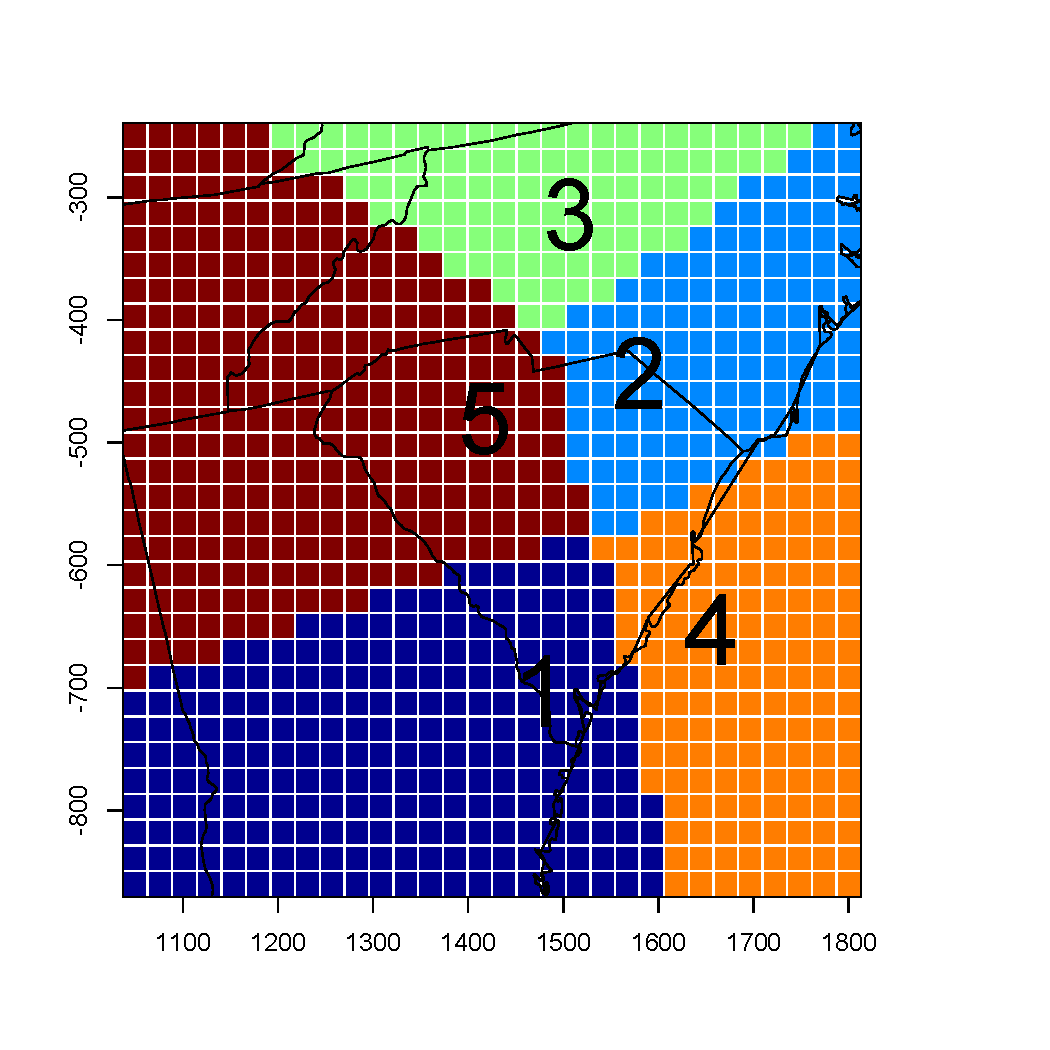
\includegraphics[width=0.54\linewidth]{./plots/pot/example-partition-1.pdf}
    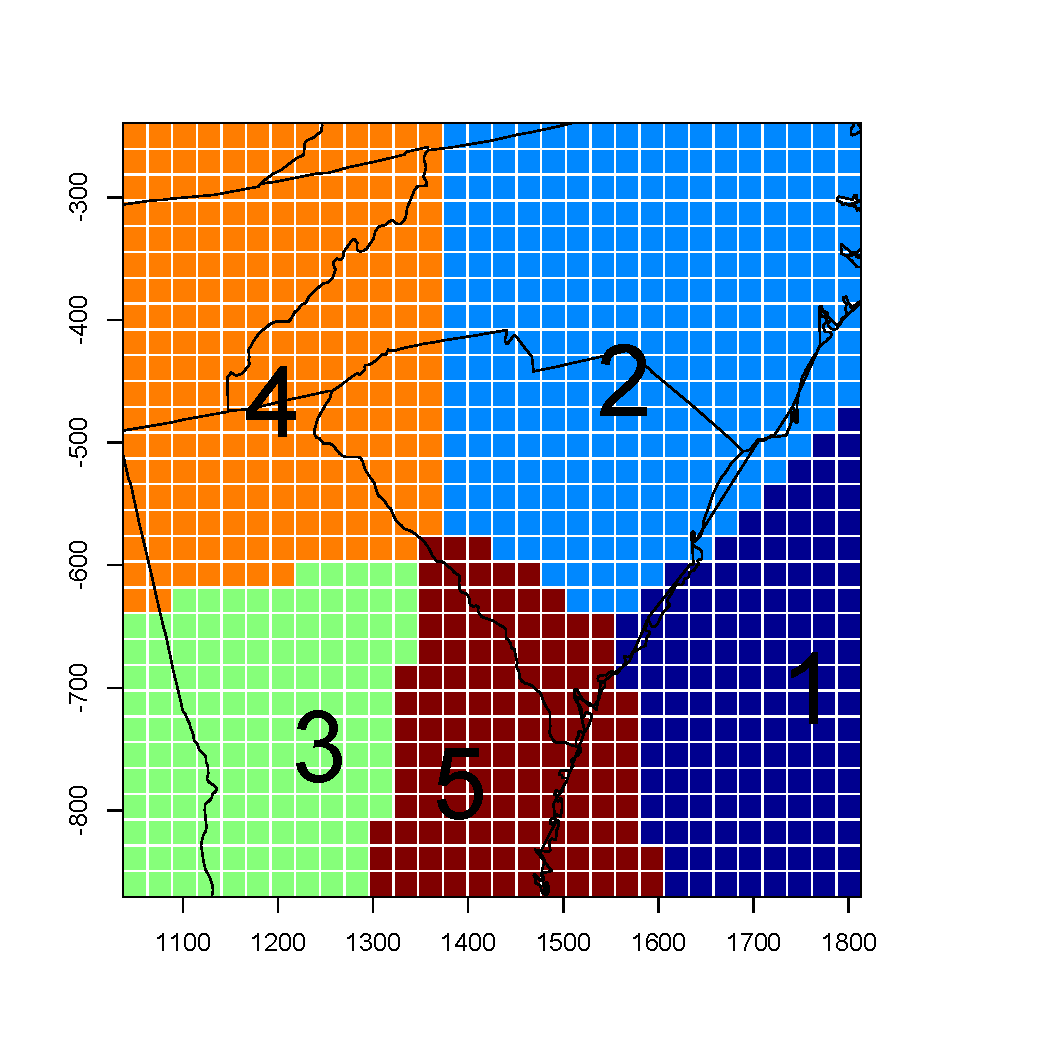
\includegraphics[width=0.54\linewidth]{./plots/pot/example-partition-2.pdf}
    \caption{Two sample partitions (number is at partition center)}
    \end{figure}
\end{frame}


\begin{frame}{$\chi(\bh)$ plot}
  \vspace{-2em}
  \centering
  \begin{figure}
  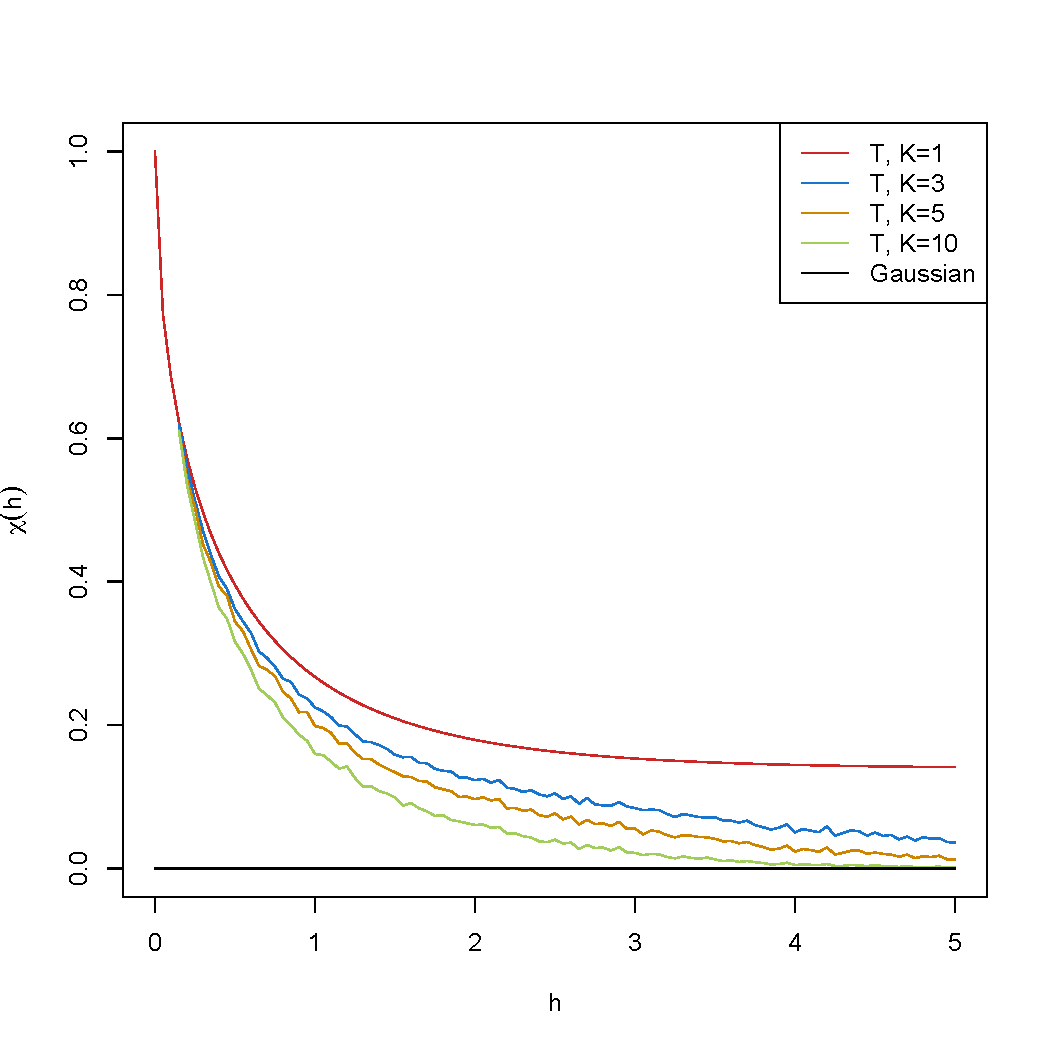
\includegraphics[width=.7\linewidth]{./plots/pot/chi-h.pdf}\\[-0.4in]
  \caption{$\chi$ plot for different data settings}
  \end{figure}
\end{frame}

\begin{frame}{Sample simulated datasets}
  \centering
  \begin{figure}
  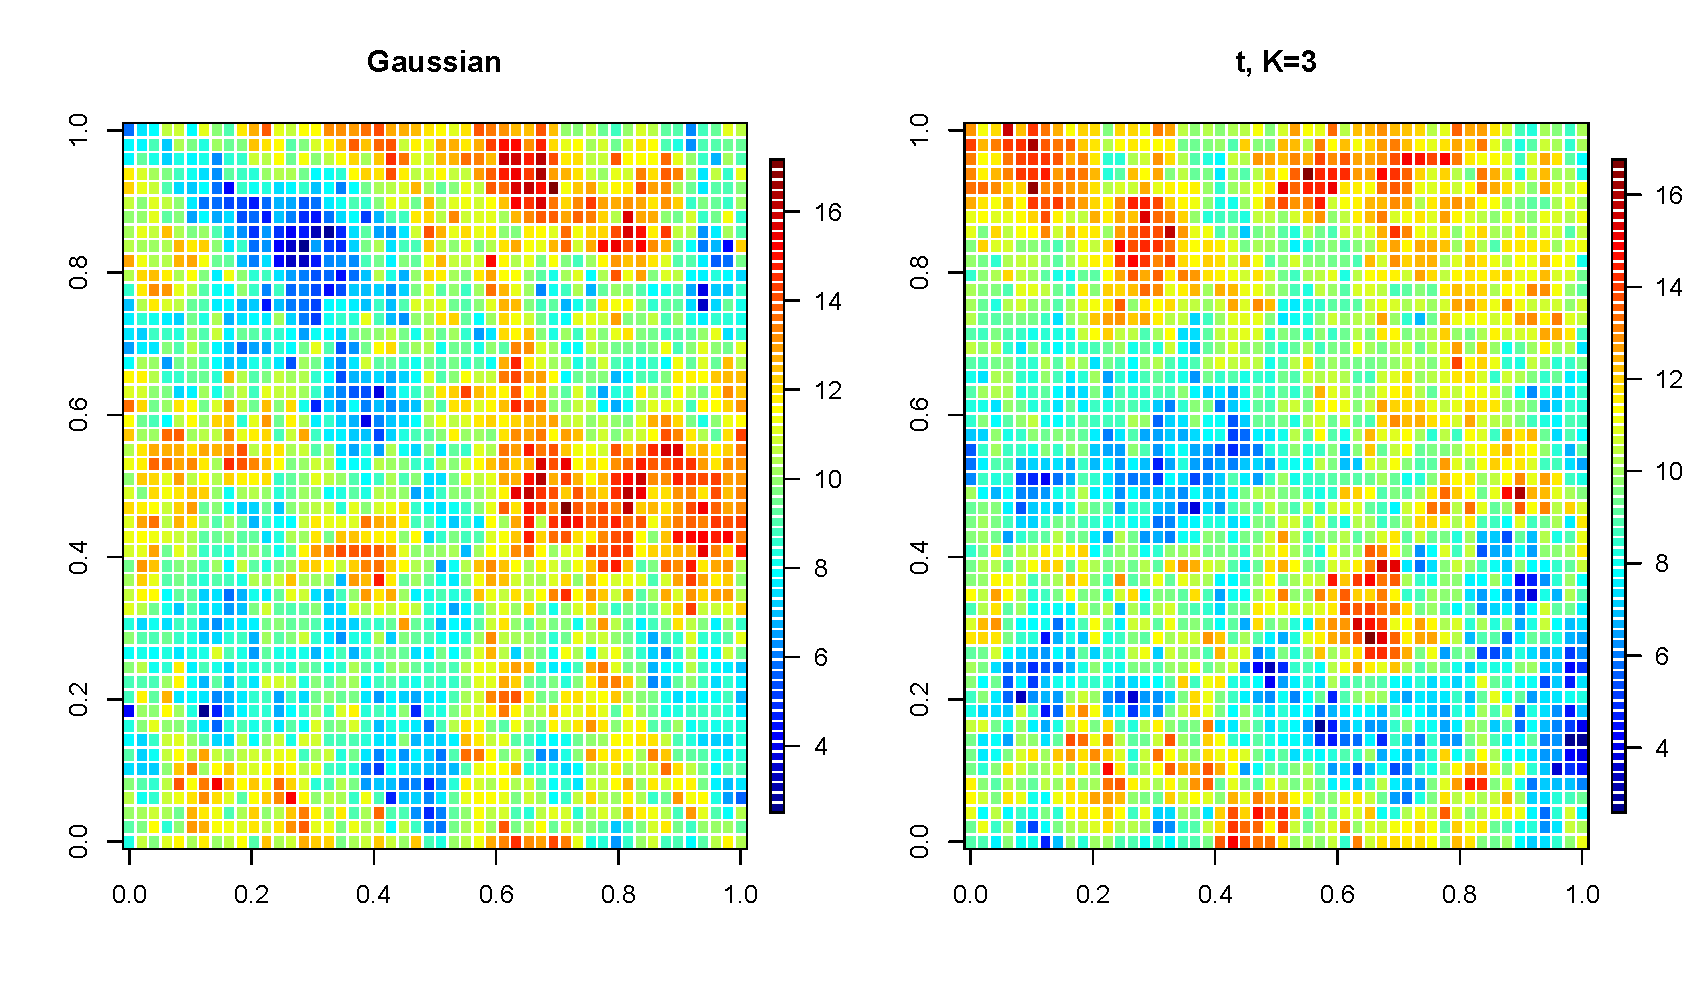
\includegraphics[width=1\linewidth]{./plots/pot/gauss-vs-t3.pdf}
  \caption{Gaussian and $t$ with 3 partitions}
  \end{figure}
\end{frame}

\begin{frame}{Sample simulated datasets}
  \centering
  \begin{figure}
  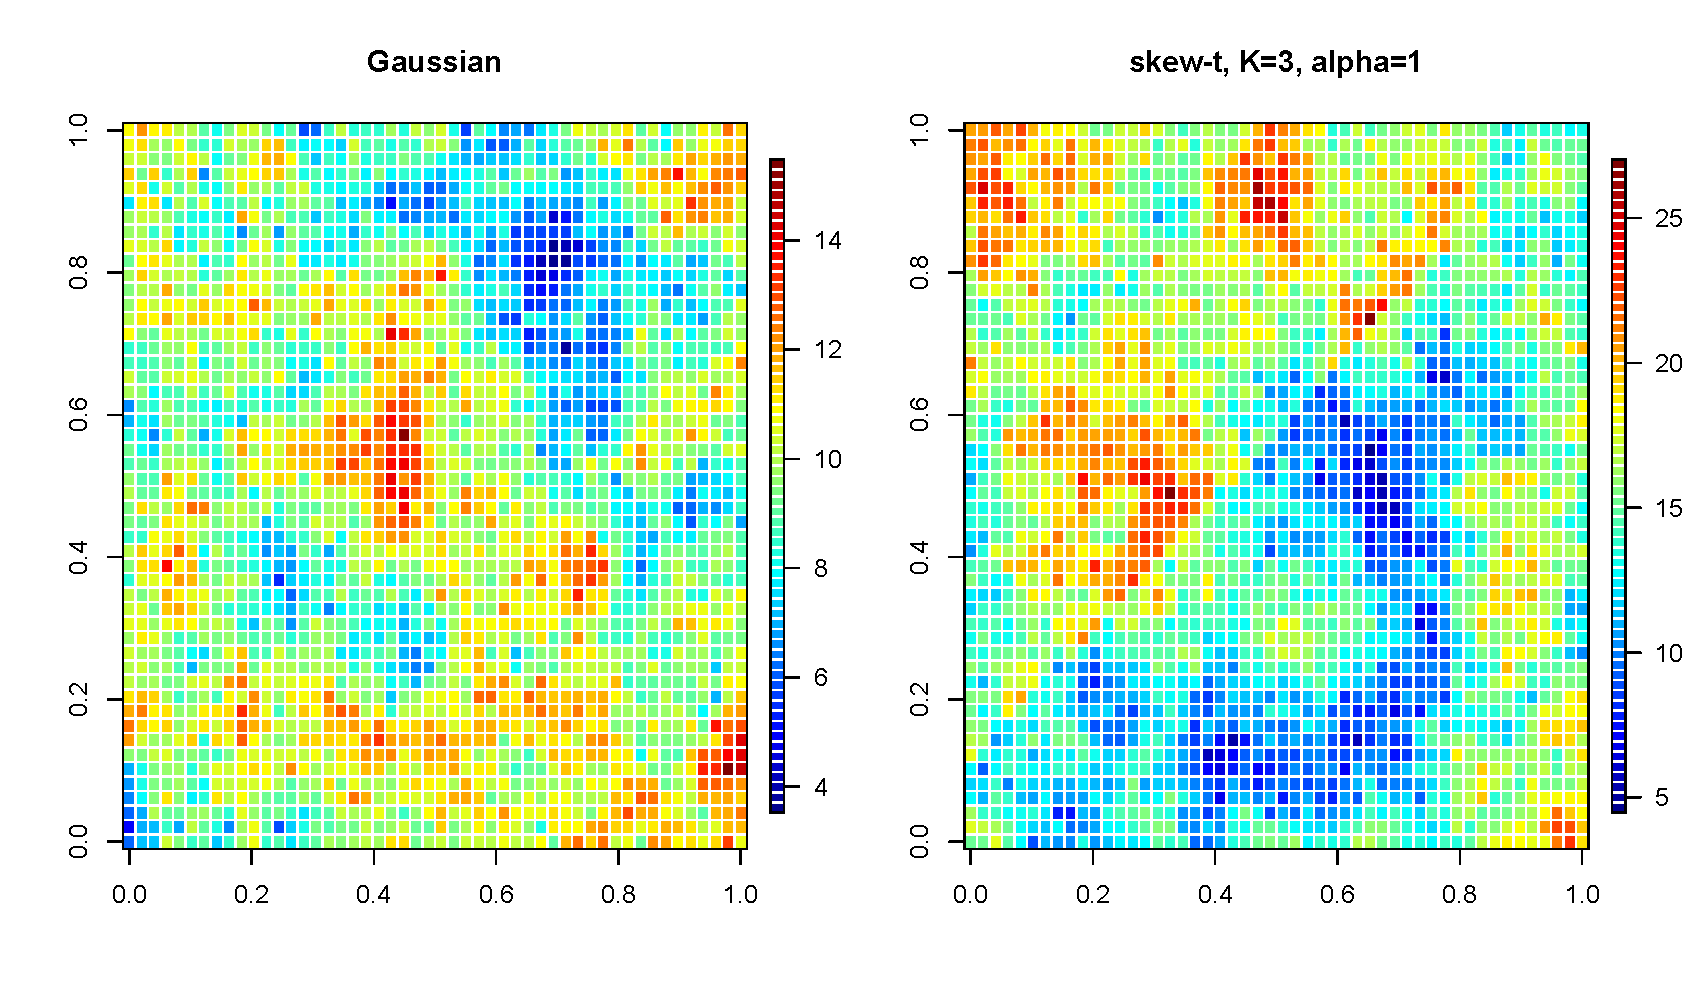
\includegraphics[width=1\linewidth]{./plots/pot/gauss-vs-skew-t3.pdf}
  \caption{Gaussian and skew-$t$ with 3 partitions}
  \end{figure}
\end{frame}

\begin{frame}{Extension to space-time data}
  \begin{itemize} \setlength{\itemsep}{0.5em}
    \item We extend our previous model to be
    \begin{align*}
      Y_t(\bs) = \bX_t(\bs)^T \bbeta + \lambda \sigma_t(\bs) | z_t(\bs) | + \sigma_t(\bs) v_t(\bs)
    \end{align*}
    where $t = 1, \ldots, T$ denotes the day of each observation.
    \item We incorporate an AR(1) time series on $\bw^*_{tk} = (w^*_{tk1}, w^*_{tk2})$, $z_{tk}$, and $\sigma^*_{tk}$ where
    \begin{align*}
      w^*_{tki} &= \Phi^{-1}\left[ \frac{w_{tki} - \min(\bs_i)}{ \text{range}(\bs_i)}\right] \quad i = 1, 2 \\
      \sigma^{2*}_t(\bs) &= \Phi^{-1}\{ \text{IG}[\sigma^2_t(\bs)] \}
    \end{align*}
    are transformations to $\calR^2$
  \end{itemize}
\end{frame}

\begin{frame}{MCMC details}
  \begin{itemize} \setlength{\itemsep}{0.5em}
    \item Three main steps:
    \begin{enumerate}[1.]
      \item Impute censored data below $T$
      \item Update parameters with standard random walk Metropolis Hastings or Gibbs sampling
      \item Make spatial predictions
    \end{enumerate}
    \item Priors are selected to be conjugate when possible
  \end{itemize}
\end{frame}

\begin{frame}{Simulation study}
  \begin{itemize} \setlength{\itemsep}{0.5em}
    \item 6 different data settings:
    \begin{itemize}
      \item Gaussian vs $t$ vs skew-$t$ marginal distribution
        \item $K=1$ partition vs $K=5$ partitions
    \end{itemize}
    \item 5 different models:
    \begin{itemize}
      \item Gaussian vs skew-$t$ marginal distribution
      \item $K = 1$ partition vs $K = 5$ partitions
    \end{itemize}
    \item Brier score used to determine model that gives best fit
  \end{itemize}
\end{frame}

% \begin{frame}{Quantile score for cross-validation}
%   \begin{itemize} \setlength{\itemsep}{0.5em}
%     \item The quantile score for the $\tau$th quantile is
%     \begin{align*}
%       2 \{ I[y < \widehat{q}(\tau)] - \tau\} (\widehat{q} - y)
%     \end{align*}
%     where:
%     \begin{itemize}
%       \item $y$ is a test set value
%       \item $\widehat{q}(\tau)$ is the estimated $\tau$th quantile
%     \end{itemize}
%   \end{itemize}
% \end{frame}

\begin{frame}{Brier score}
  \begin{itemize} \setlength{\itemsep}{0.5em}
  \item The Brier score for predicting exceedance of threshold $c$ is
  \begin{align*}
    [e(c) - P(c)]^2
  \end{align*}
  where
  \begin{itemize}
    \item $y$ is a test set value
    \item $e(c) = I[y > c]$
    \item $P(c)$ is the predicted probability of exceeding $c$
  \end{itemize}
  \item Relative Brier scores:
  \begin{align*}
    \text{BS}_\text{rel} = \frac{ \text{BS}_\text{method}}{ \text{BS}_\text{Gaussian}}
  \end{align*}
  \end{itemize}
\end{frame}

\begin{frame}{Simulation study results}
\centering
  \begin{figure}
    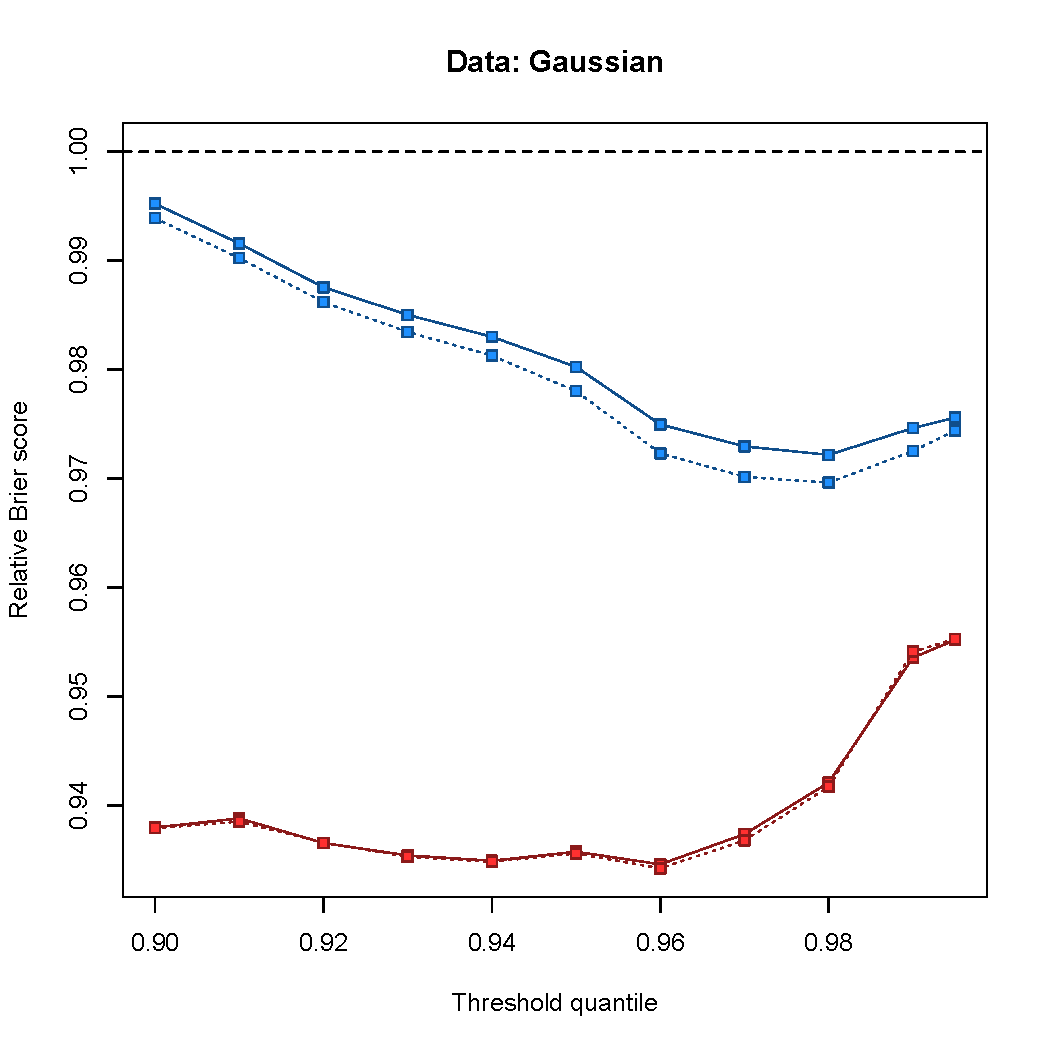
\includegraphics[width=0.45\linewidth]{./plots/pot/bs-sim-gaus.pdf}
    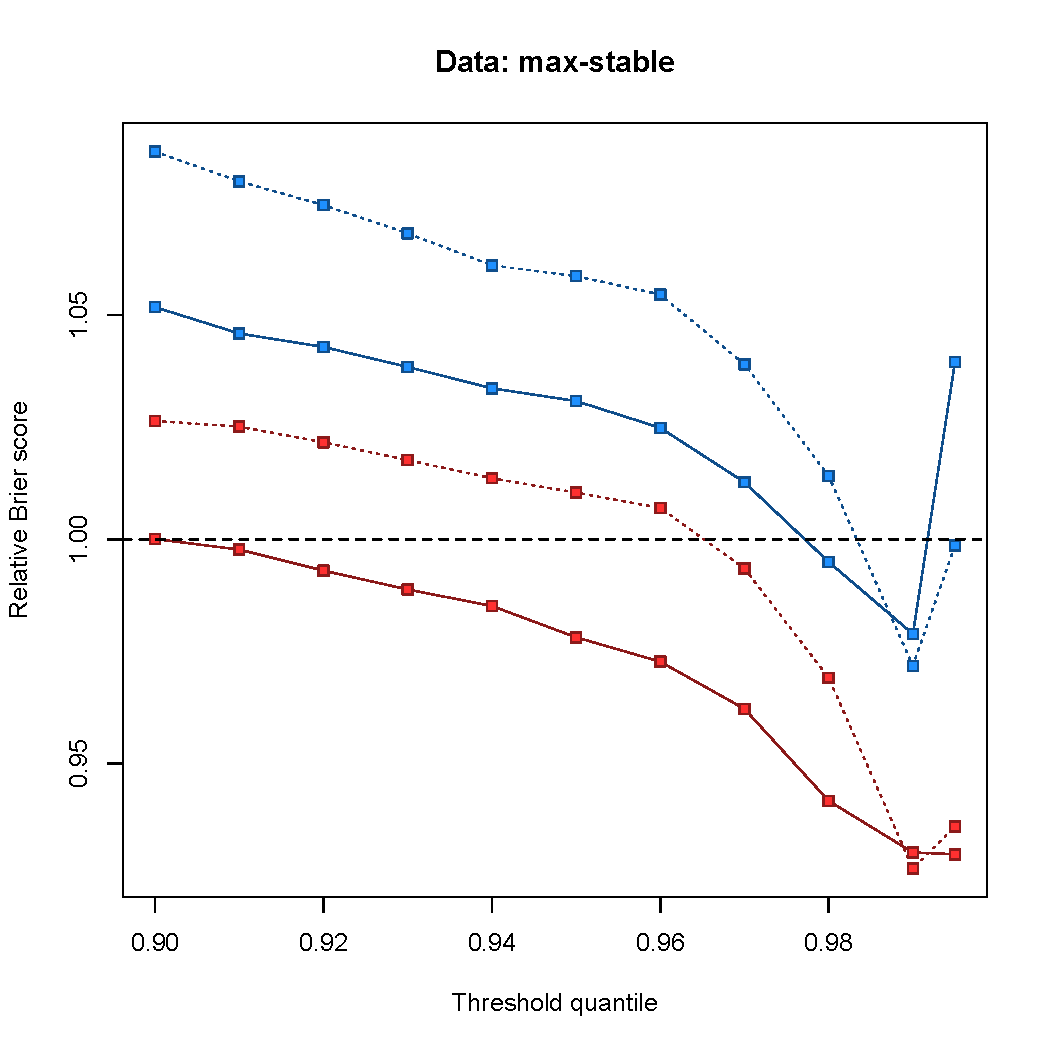
\includegraphics[width=0.45\linewidth]{./plots/pot/bs-sim-max.pdf} \\
    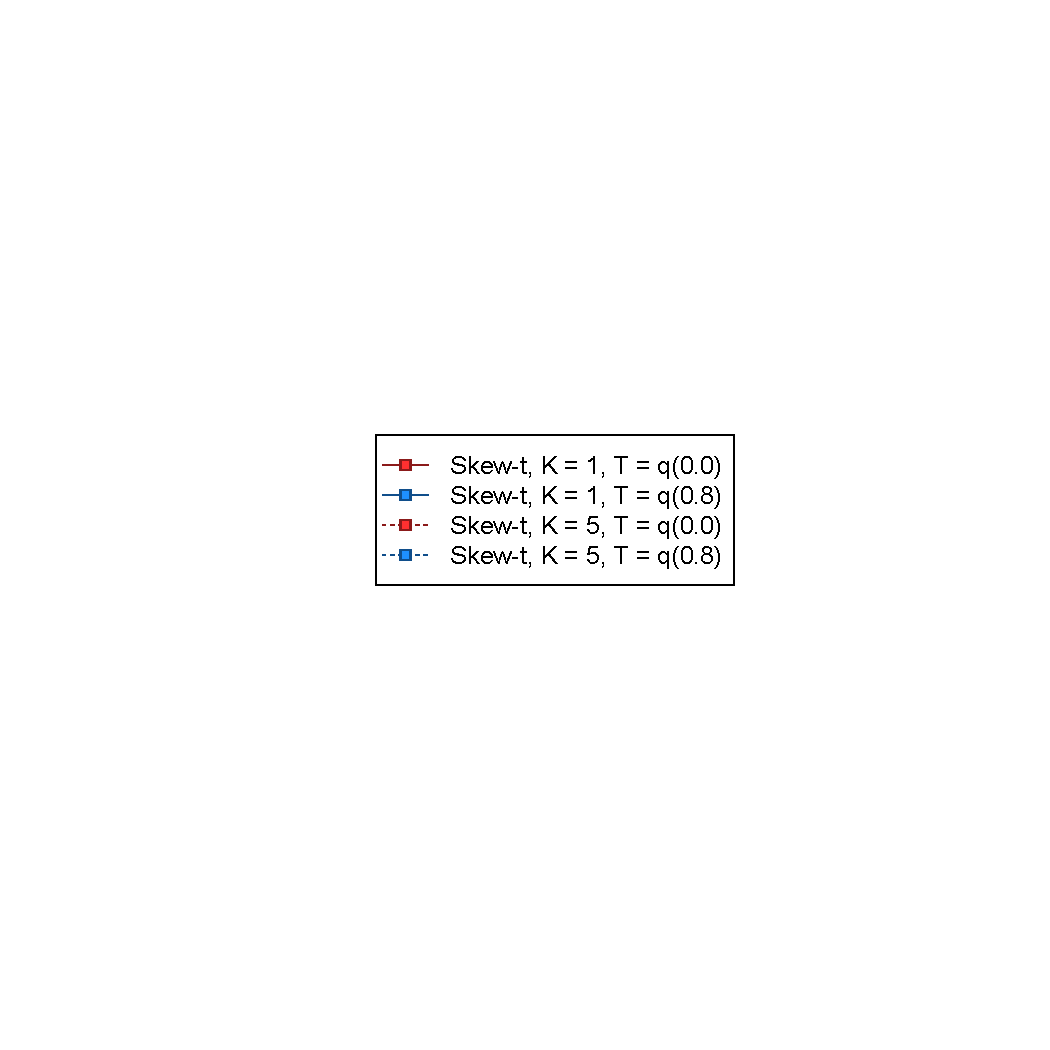
\includegraphics[width=0.3\linewidth, trim=2in 3.25in 2in 3in]{./plots/pot/bs-sim-legend.pdf}
    \caption{Relative Brier score results}
  \end{figure}
\end{frame}

\begin{frame}{Simulation study results}
\centering
  \begin{figure}
    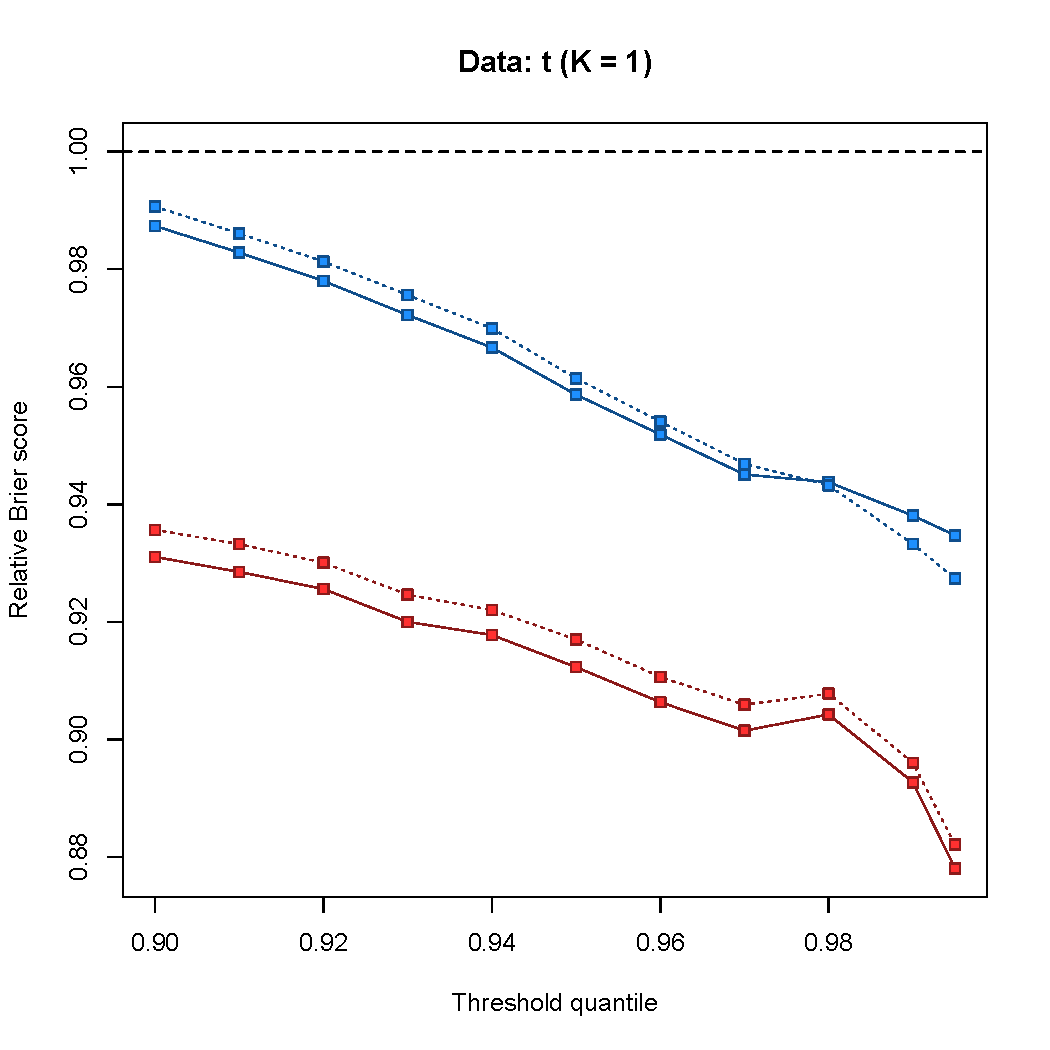
\includegraphics[width=0.45\linewidth]{./plots/pot/bs-sim-t1.pdf}
    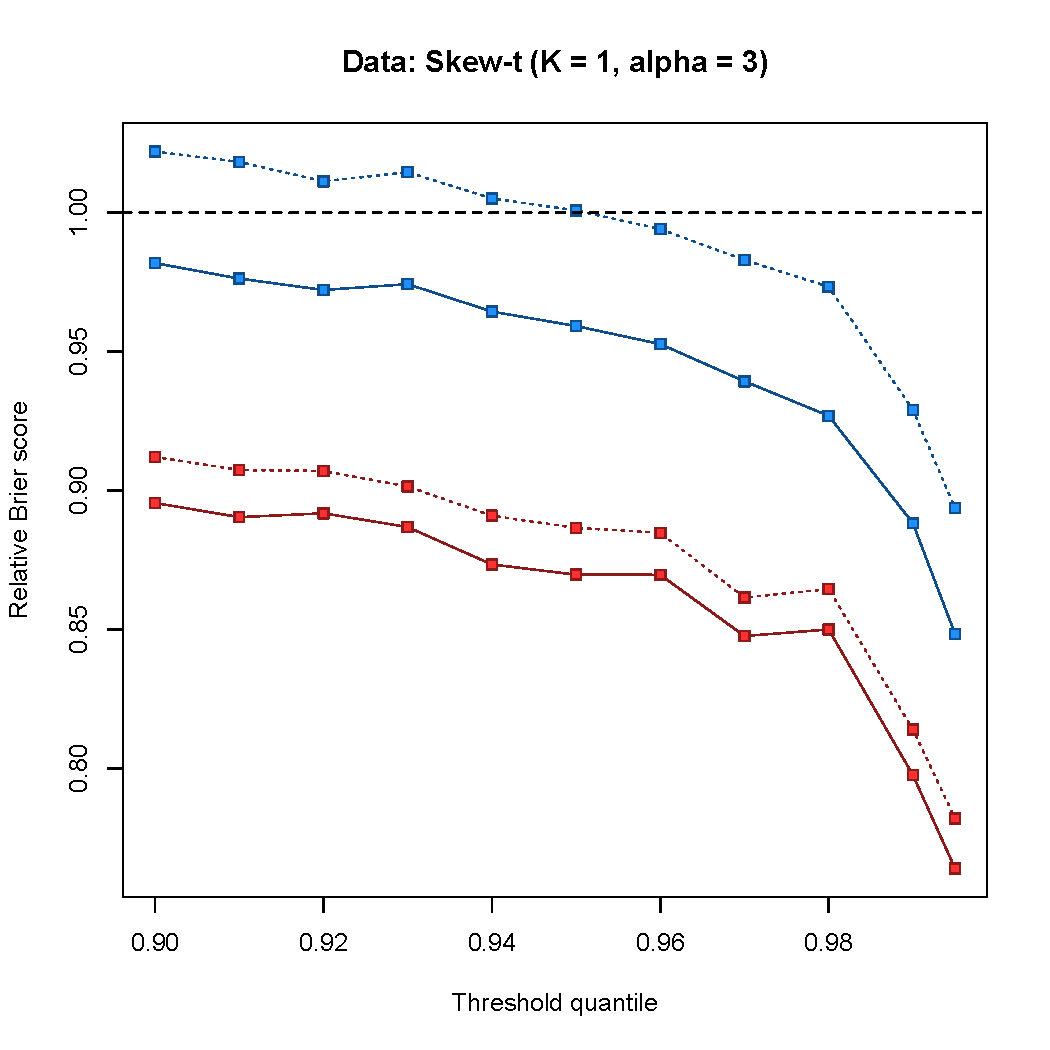
\includegraphics[width=0.45\linewidth]{./plots/pot/bs-sim-st1.pdf} \\
    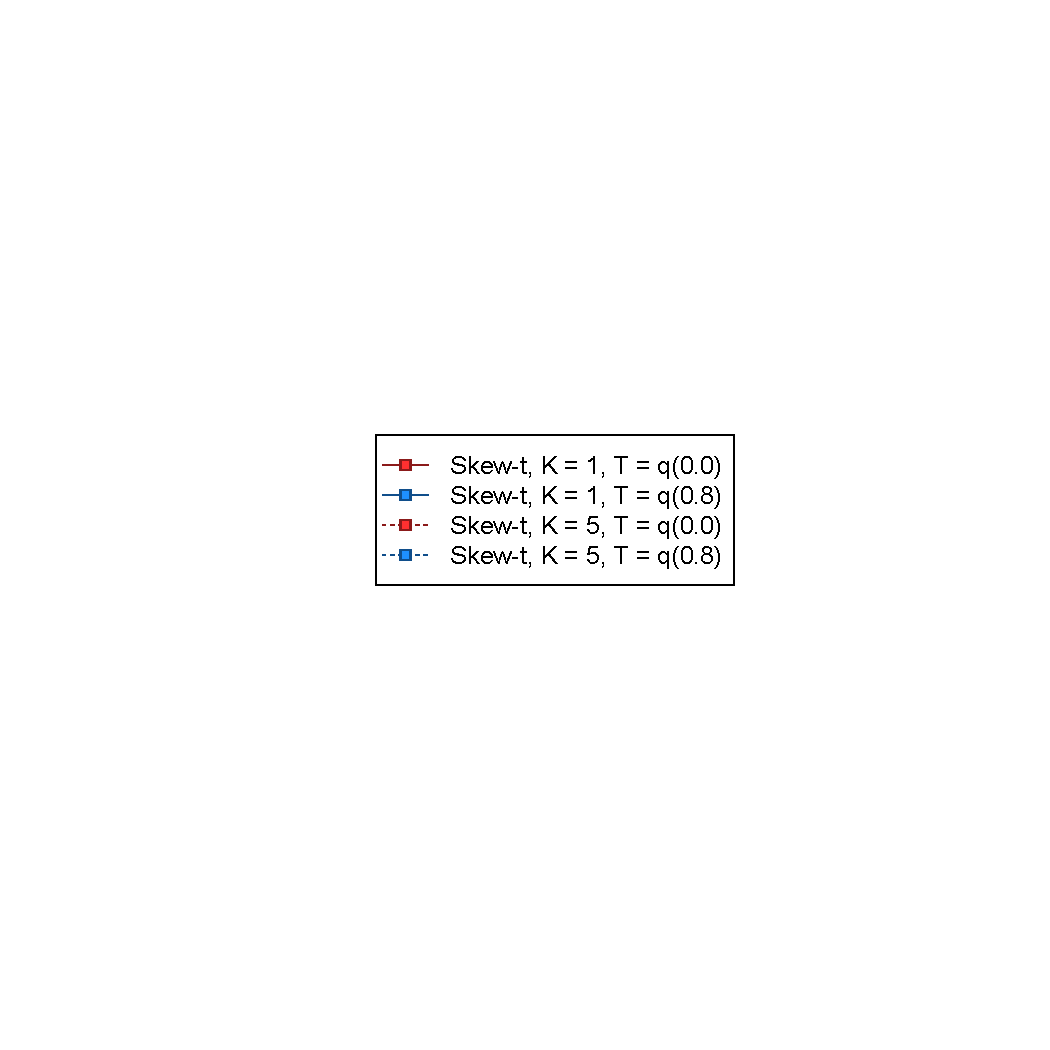
\includegraphics[width=0.3\linewidth, trim=2in 3.25in 2in 3in]{./plots/pot/bs-sim-legend.pdf}
    \caption{Relative Brier score results}
  \end{figure}
\end{frame}

\begin{frame}{Simulation study results}
\centering
  \begin{figure}
    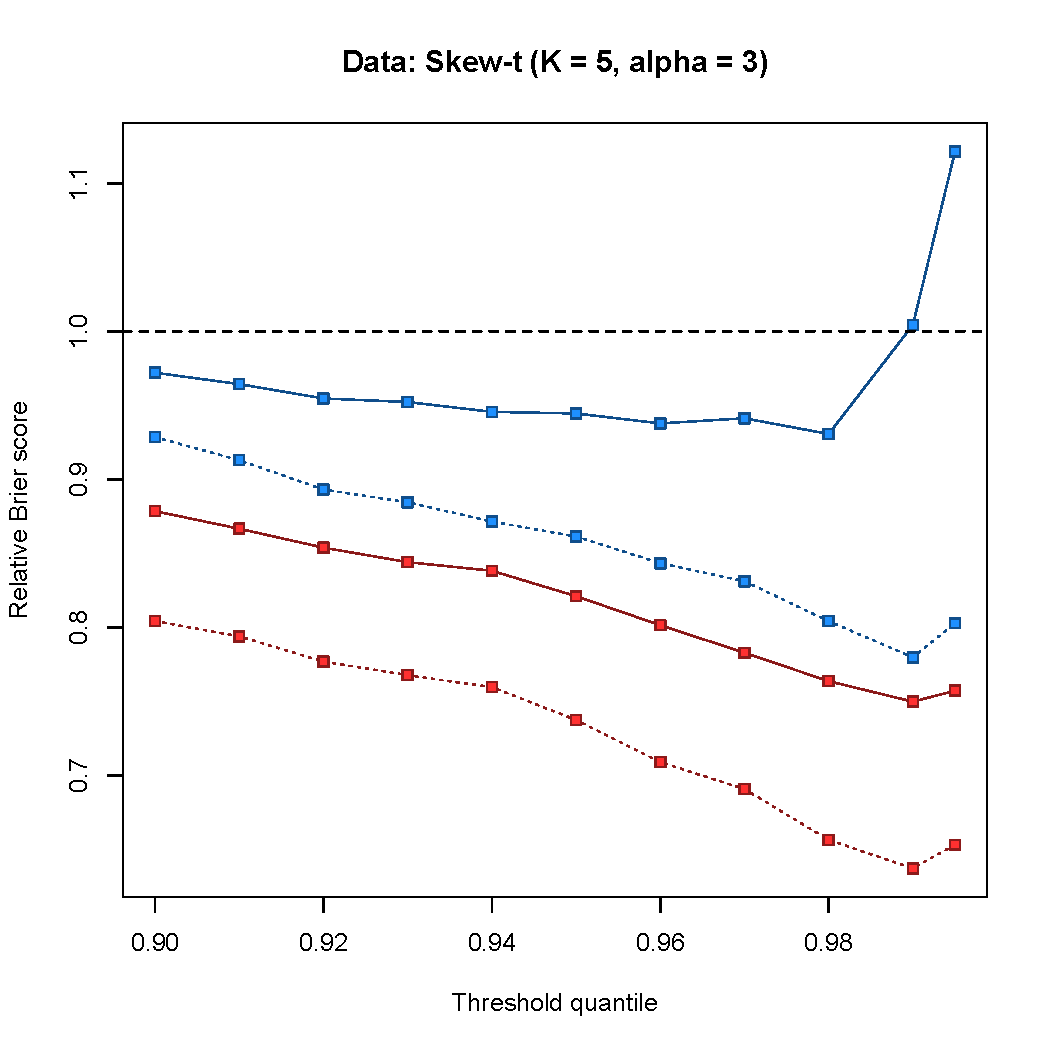
\includegraphics[width=0.45\linewidth]{./plots/pot/bs-sim-t5.pdf}
    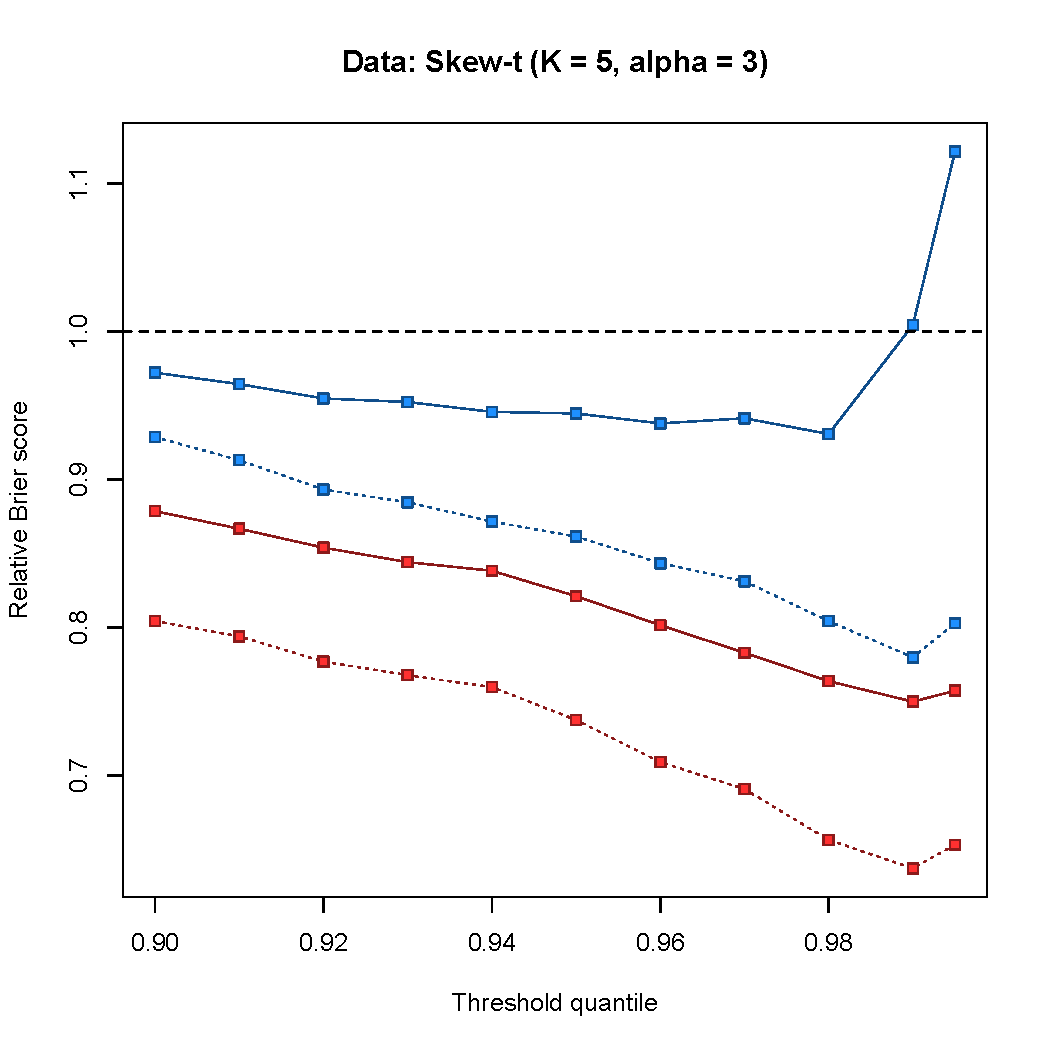
\includegraphics[width=0.45\linewidth]{./plots/pot/bs-sim-st5.pdf} \\
    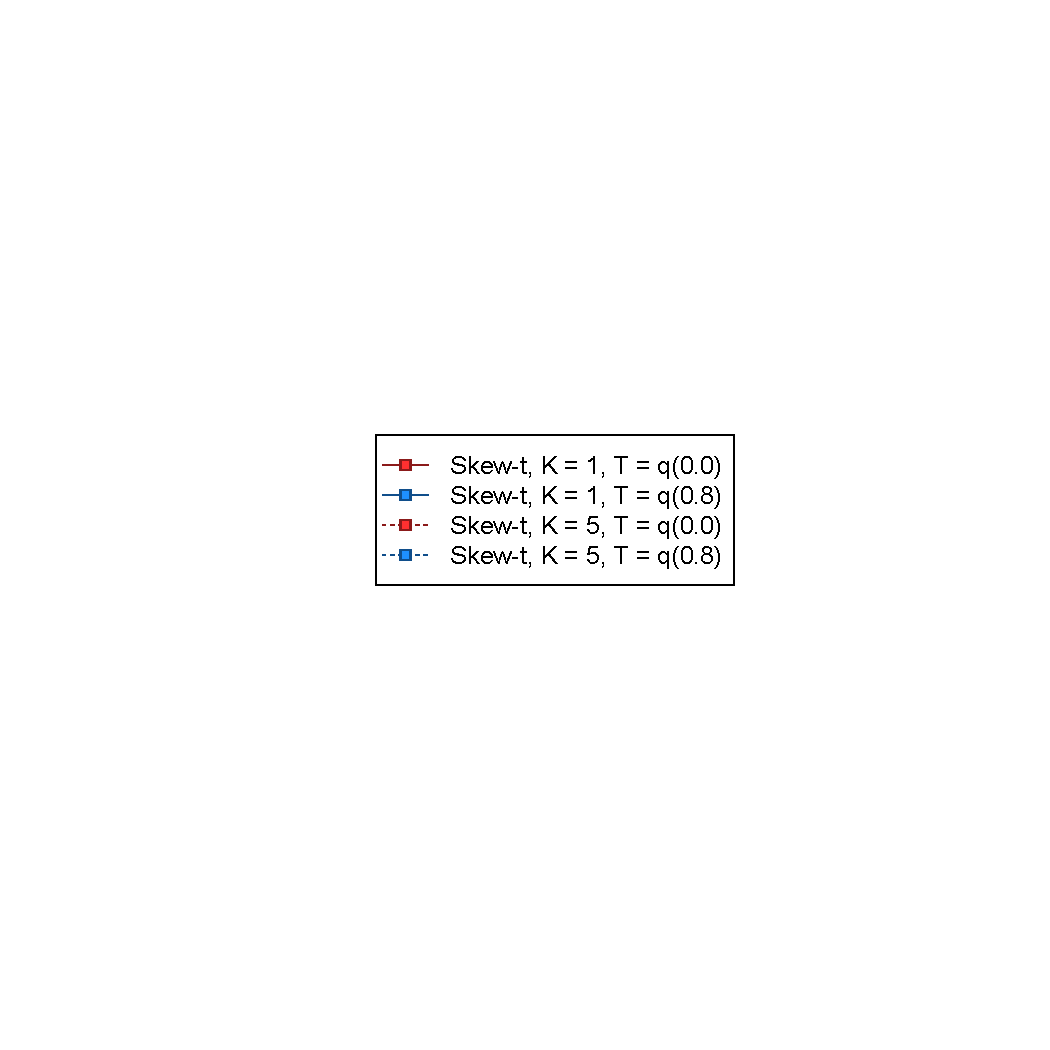
\includegraphics[width=0.3\linewidth, trim=2in 3.25in 2in 3in]{./plots/pot/bs-sim-legend.pdf}
    \caption{Relative Brier score results}
  \end{figure}
\end{frame}

\begin{frame}{Simulation study results}
  \begin{itemize} \setlength{\itemsep}{0.5em}
    \item Key findings:
    \begin{itemize}
      \item Improvement over Gaussian methods when partitioning
      \item Underestimating the number of knots has a detrimental impact
      \item In all cases, non-thresholded models perform better than thresholded models
    \end{itemize}
  \end{itemize}
\end{frame}

\begin{frame}{Data analysis}
\begin{columns}[c]
\column{.45 \linewidth}
	\begin{itemize} \setlength{\itemsep}{0.5em}
	\item Ozone measurements
	\begin{itemize}
		\item max 8-hour ozone measurements
		\item data from 1089 sites
		\item July 2005
	\end{itemize}
  \item We take a stratified sample of $n = 800$ sites:
  \begin{itemize}
    \item 271 from northeast
    \item 96 from northwest
    \item 269 from southeast
    \item 164 from southwest
  \end{itemize}
	\end{itemize}

	\column{.55\linewidth}
	\begin{figure}
    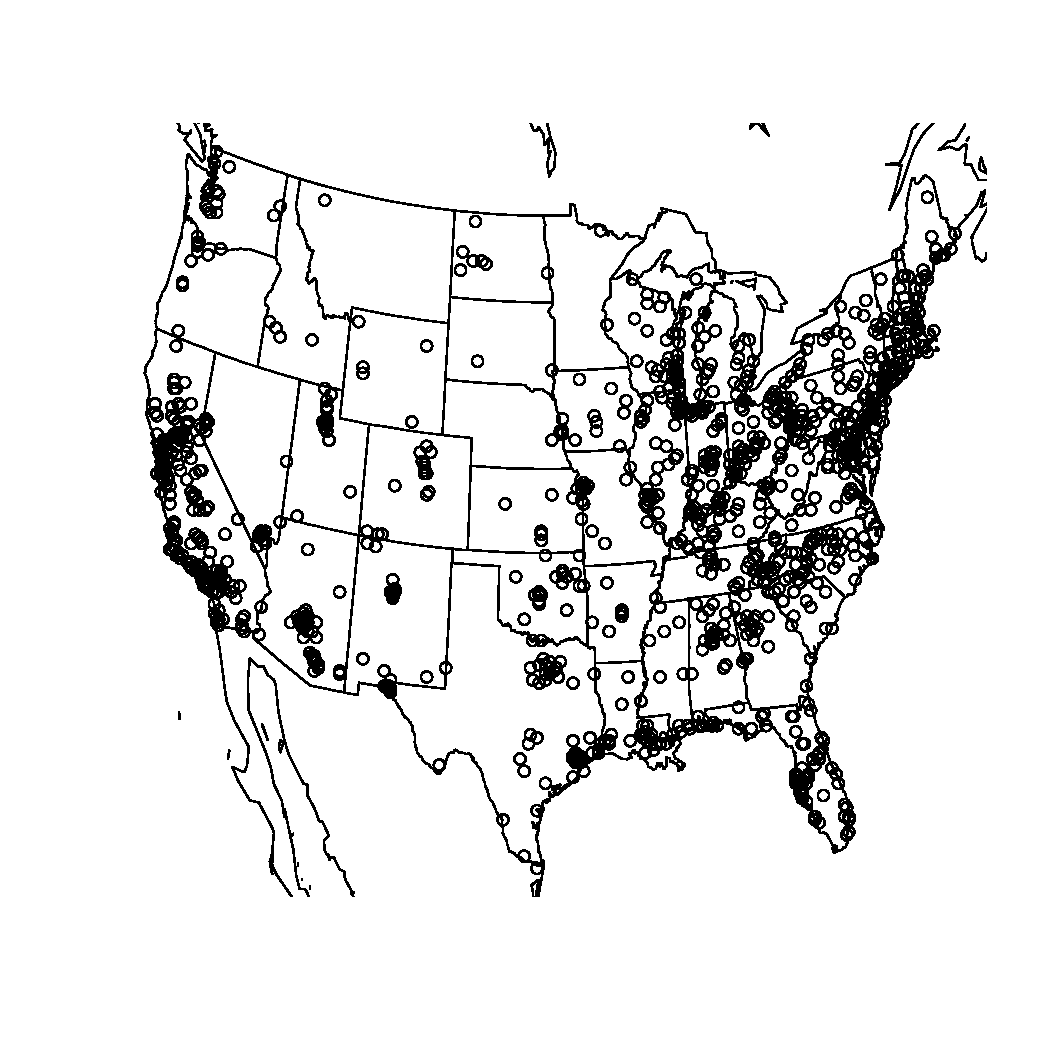
\includegraphics[width=1\linewidth]{./plots/pot/ozone_stations.pdf}
    \caption{Ozone monitoring station locations}
    \end{figure}
\end{columns}
\end{frame}

\begin{frame}{Data analysis}
  \centering
  \begin{figure}
    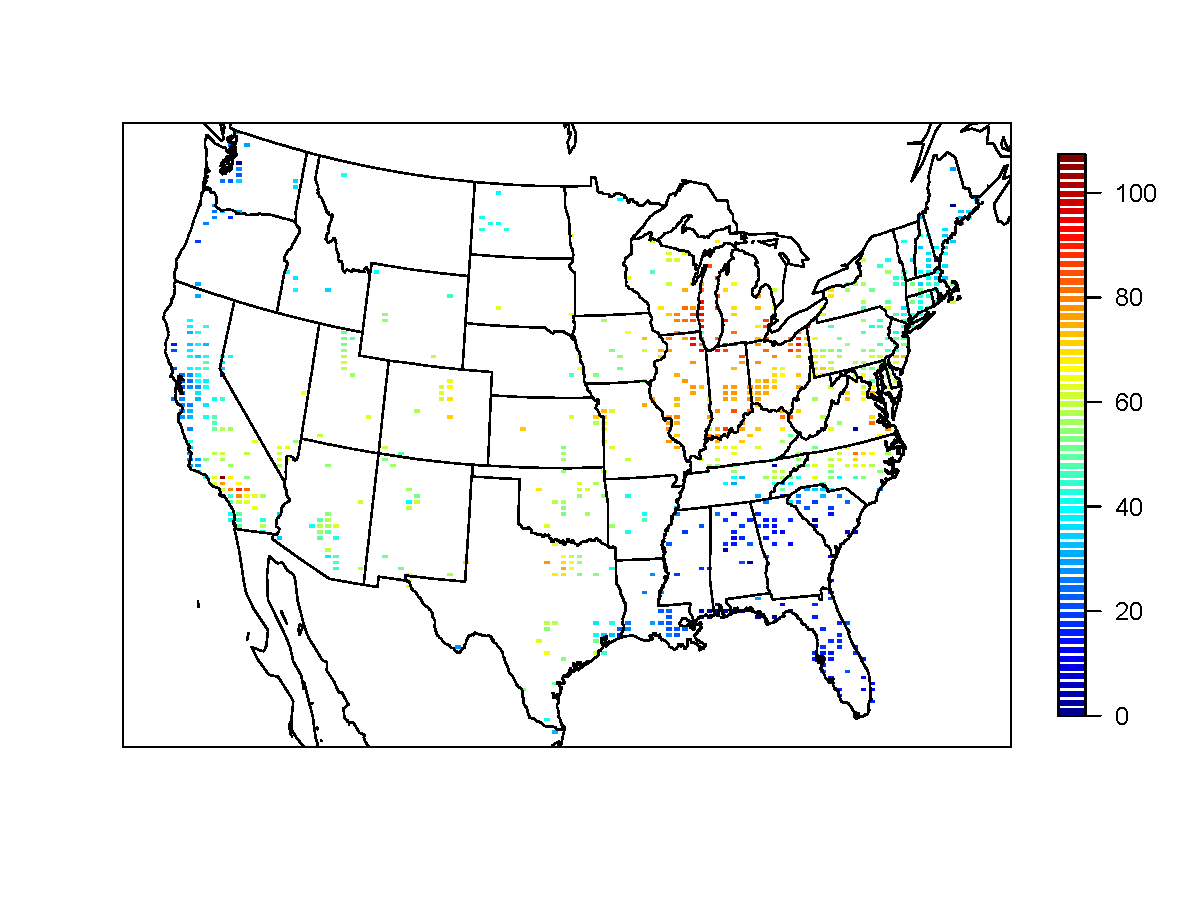
\includegraphics[width=\linewidth, trim=0 1in 0 0in ]{./plots/pot/ozone-10jul-us.pdf}
    \caption{Max 8-hour ozone measurements on July 10, 2005}
   \end{figure}

\end{frame}

\begin{frame}{Exploratory data analysis}
	\centering
  \begin{figure}
    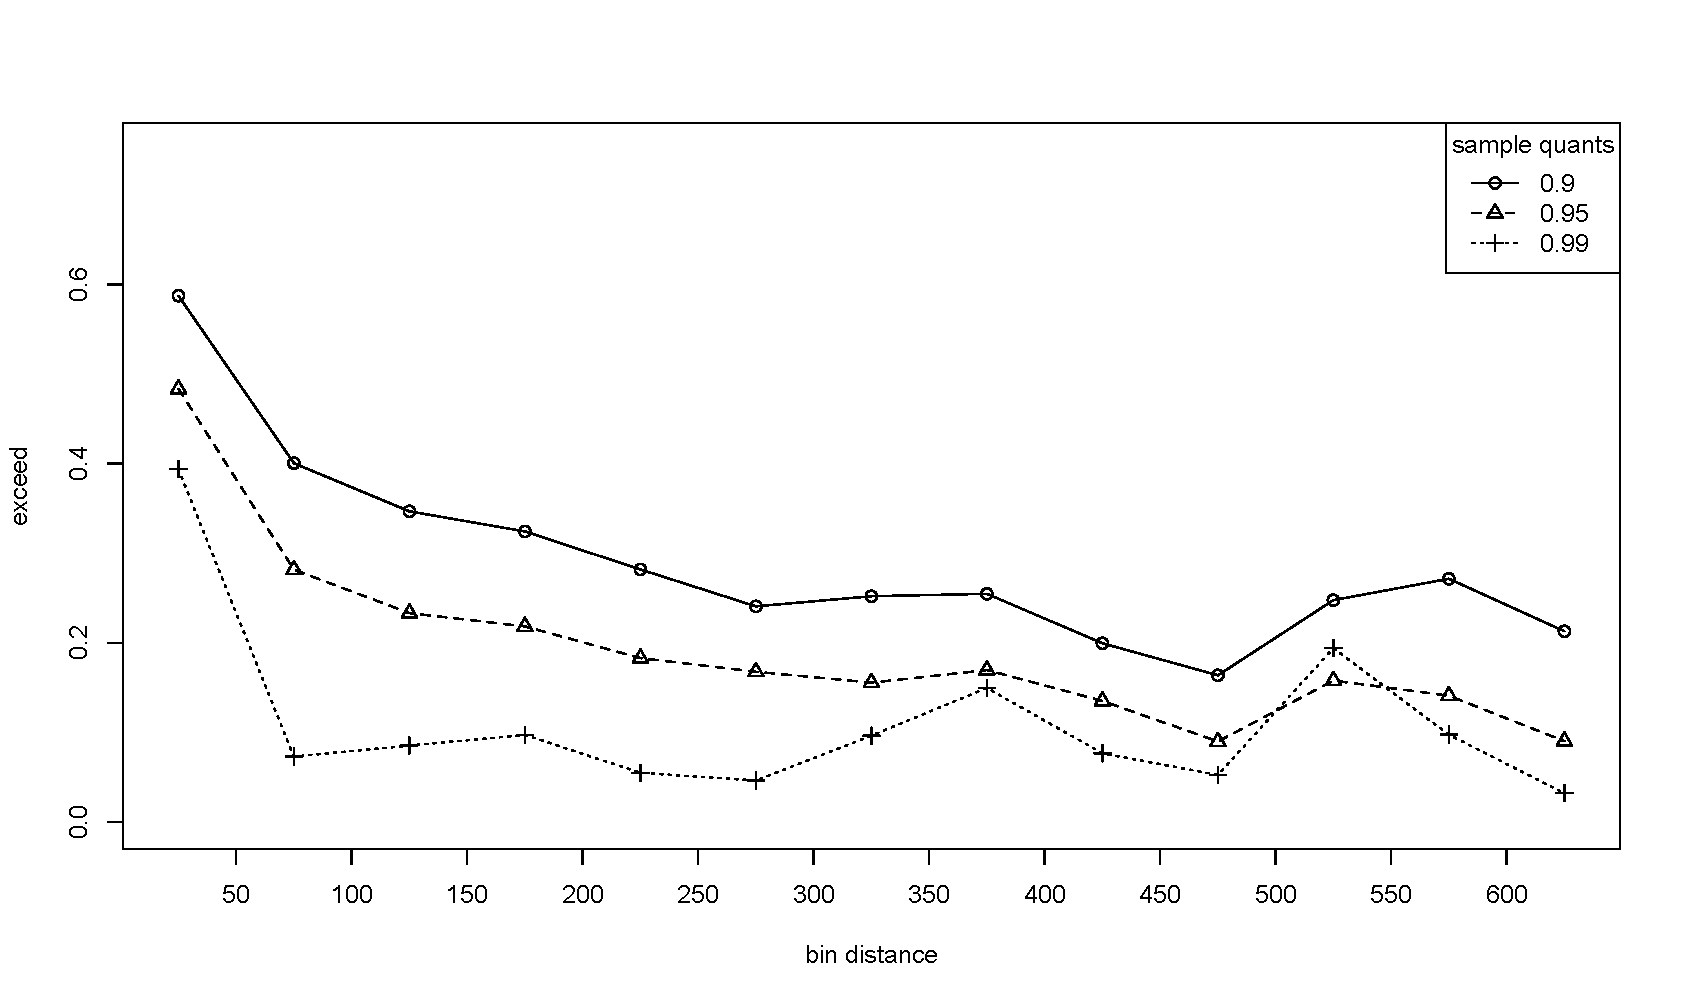
\includegraphics[width=1\linewidth]{./plots/pot/chi-plot-ozone-res.pdf}
    \caption{$\widehat{\chi}$-plot for sample quantiles of ozone observations}
  \end{figure}
\end{frame}

\begin{frame}{Model comparisons}
  \begin{itemize} \setlength{\itemsep}{0.5em}
    \item 9 different analysis methods incorporating
    \begin{itemize}
      \item Gaussian vs $t$ vs skew-$t$ marginal distribution
      \item $K=1, 5, 6, 7, 8, 9, 10, 15$ partitions
      \item Thresholding at $T=0, 50, 75$, and $85$ ppb
    \end{itemize}
    \item All methods use a \Matern or exponential covariance ($\nu = 0.5$)
    \item Compare quantile and Brier scores using two-fold cross validation (Gneiting and Raftery, 2007)
    \item Mean function modeled as
    \begin{align*}
    	\beta_0 + \beta_1 \cdot \text{CMAQ}
    \end{align*}
   \end{itemize}
\end{frame}

\begin{frame}{Two-fold cross-validation results}
  \centering
  \begin{figure}
    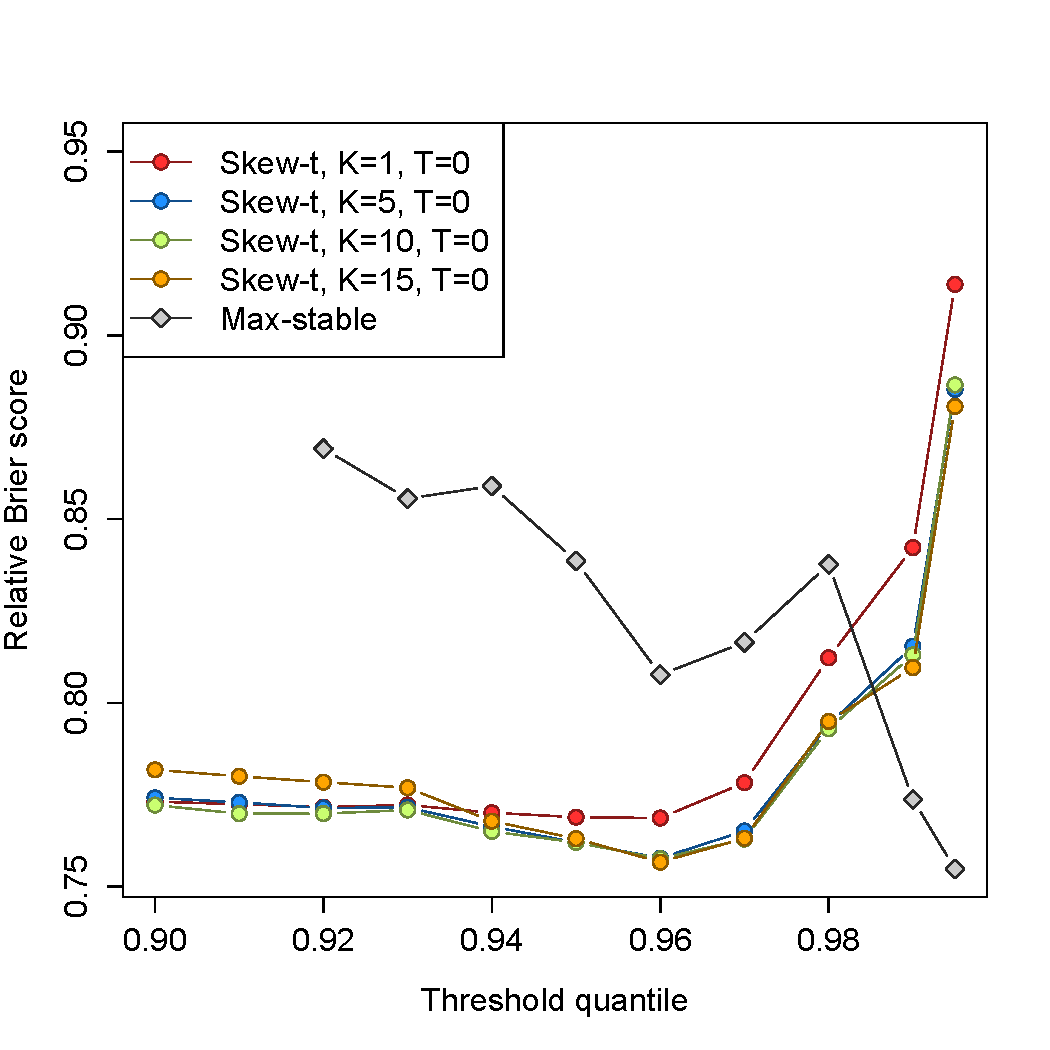
\includegraphics[width=0.45\linewidth]{./plots/pot/bs-ozone-1.pdf}
    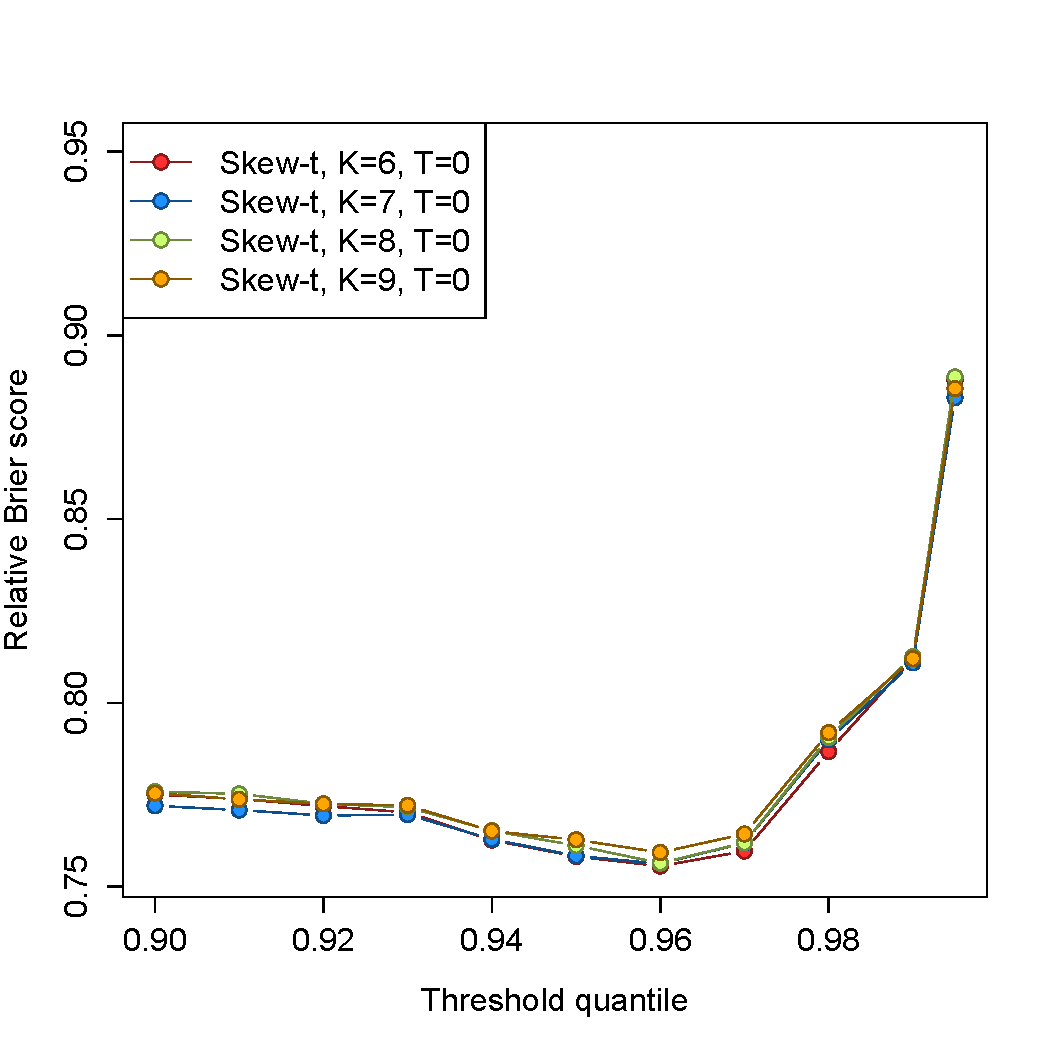
\includegraphics[width=0.45\linewidth]{./plots/pot/bs-ozone-2.pdf} \\
    \caption{Relative Brier score results}
  \end{figure}
\end{frame}

\begin{frame}{Two-fold cross-validation results}
  \begin{itemize} \setlength{\itemsep}{0.5em}
    \item Key findings:
    \begin{itemize}
      \item Partitioning improves performance across all high thresholds.
      \item Models with anywhere from $K = 5$ to $K = 10$ partitions perform similarly
      \item In all cases, non-thresholded models perform better than thresholded models
    \end{itemize}
  \end{itemize}
\end{frame}

% % TODO: Update with new plots
% \begin{frame}{Predicted 95th quantile}
% \centering
% \begin{figure}
%     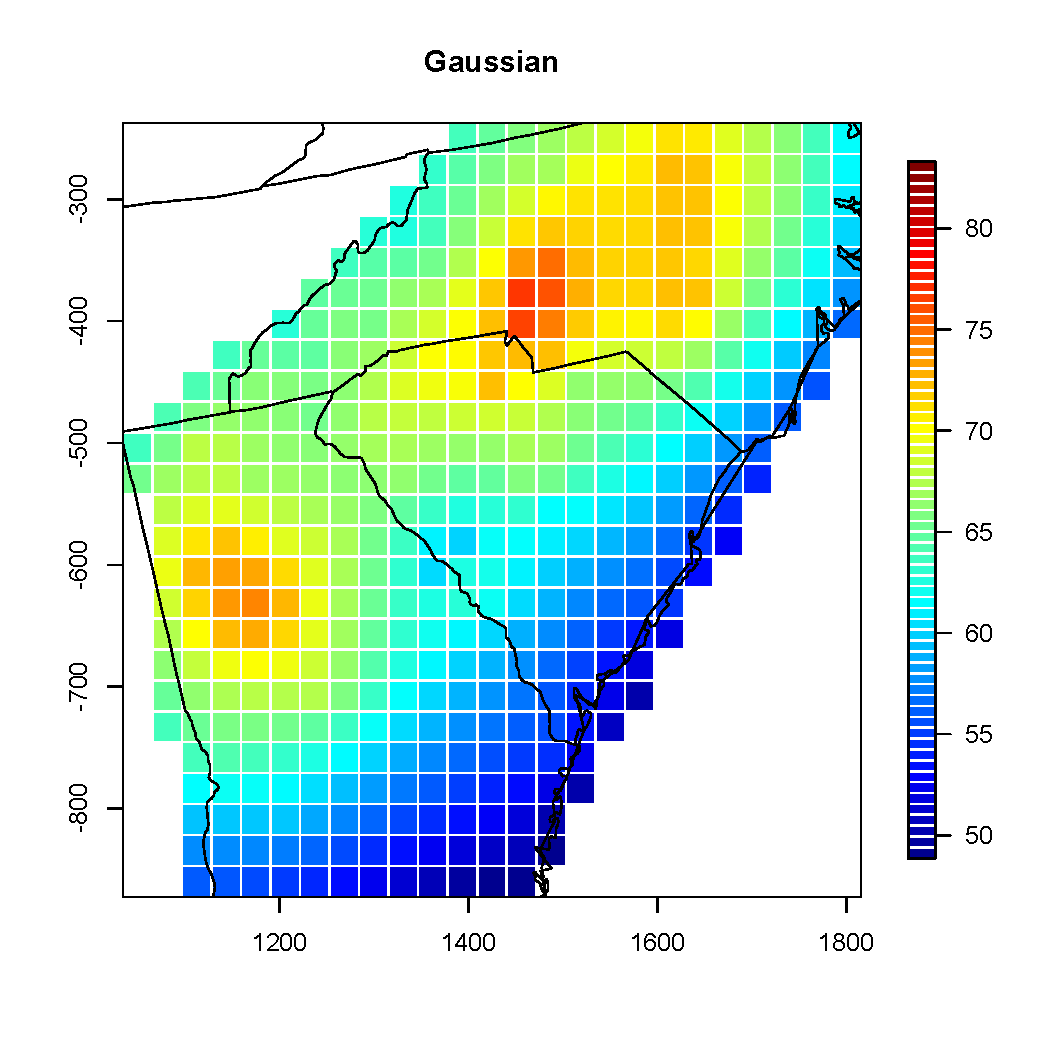
\includegraphics[width=.5\linewidth]{./plots/quantile-95-gau.pdf}
%     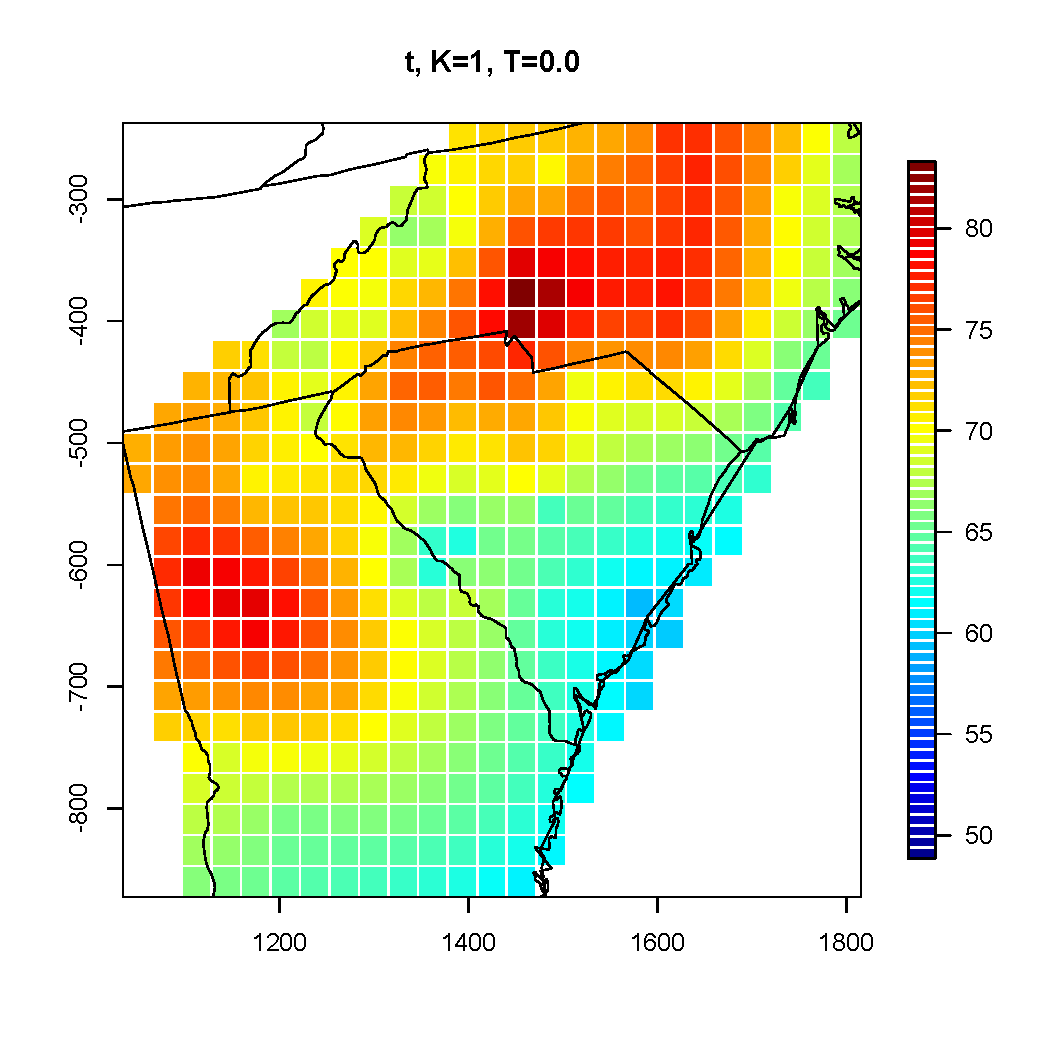
\includegraphics[width=.5\linewidth]{./plots/quantile-95-t10.pdf}
%     \caption{Predicted 95th quantile using Gaussian and $t$}
% \end{figure}
% \end{frame}

% \begin{frame}{Predicted 95th quantile}
% \centering
% \begin{figure}
%     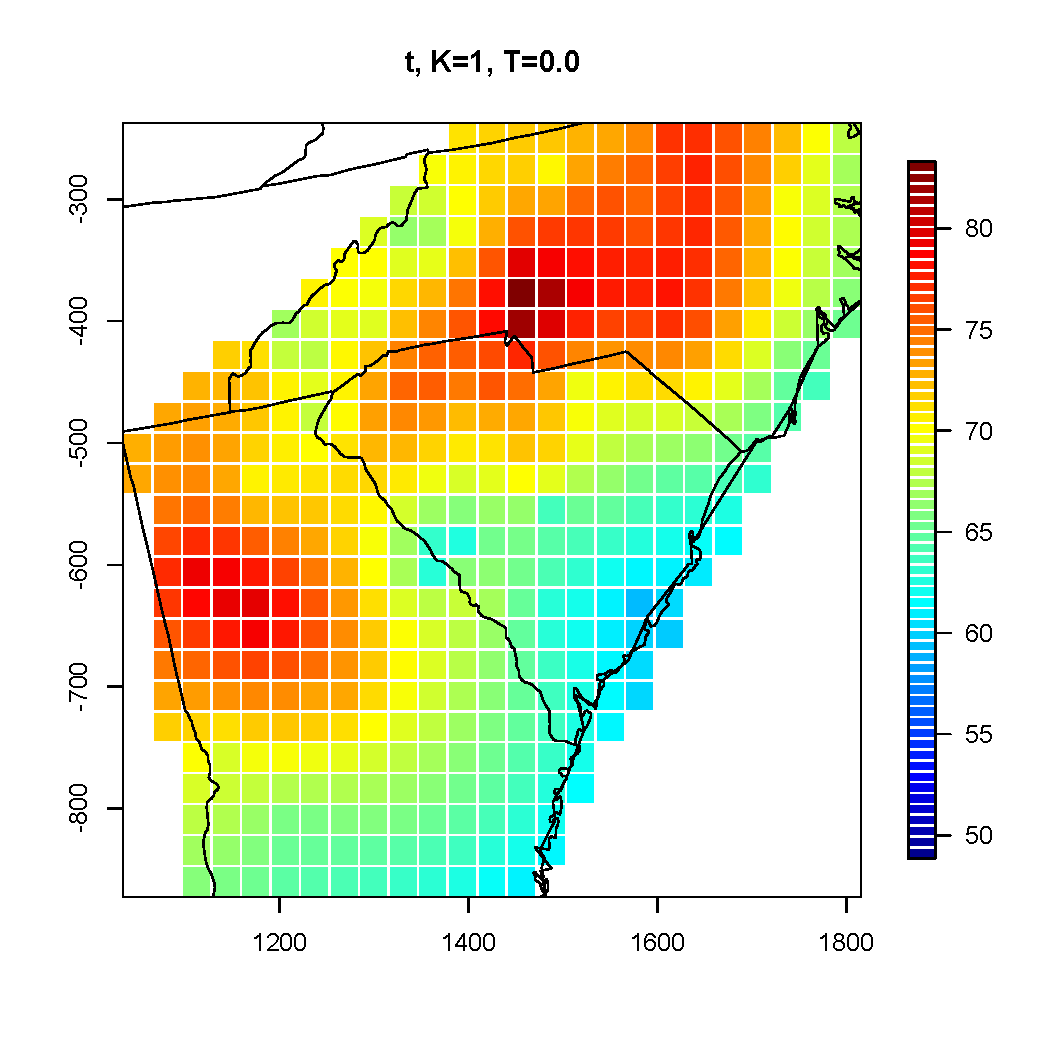
\includegraphics[width=.5\linewidth]{./plots/quantile-95-t10.pdf}
%     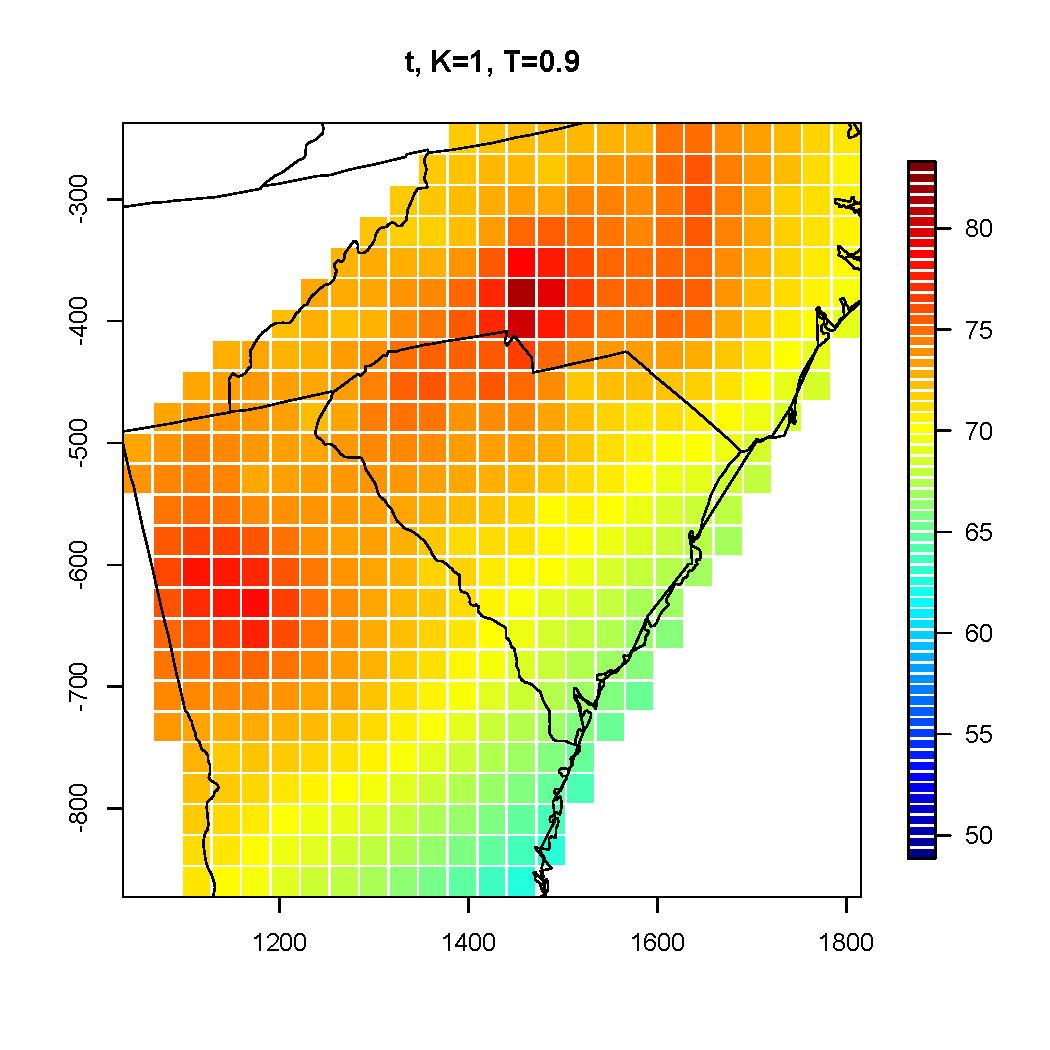
\includegraphics[width=.5\linewidth]{./plots/quantile-95-t19.pdf}
%     \caption{Predicted 95th quantile using $t$ and $t$ thresholded at $T=0.9$}
% \end{figure}
% \end{frame}

% \begin{frame}{Predicted 99th quantile}
% \centering
% \begin{figure}
%     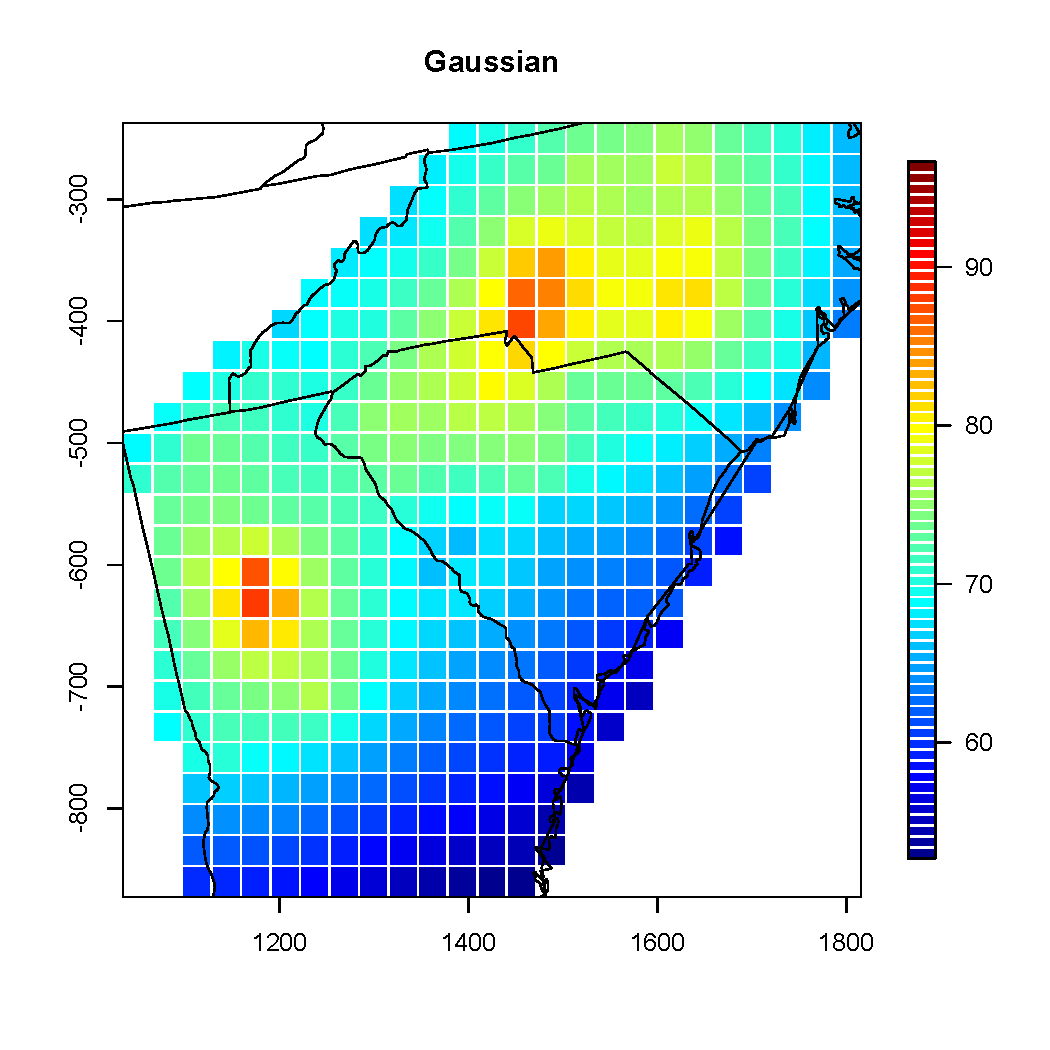
\includegraphics[width=.5\linewidth]{./plots/quantile-99-gau.pdf}
%     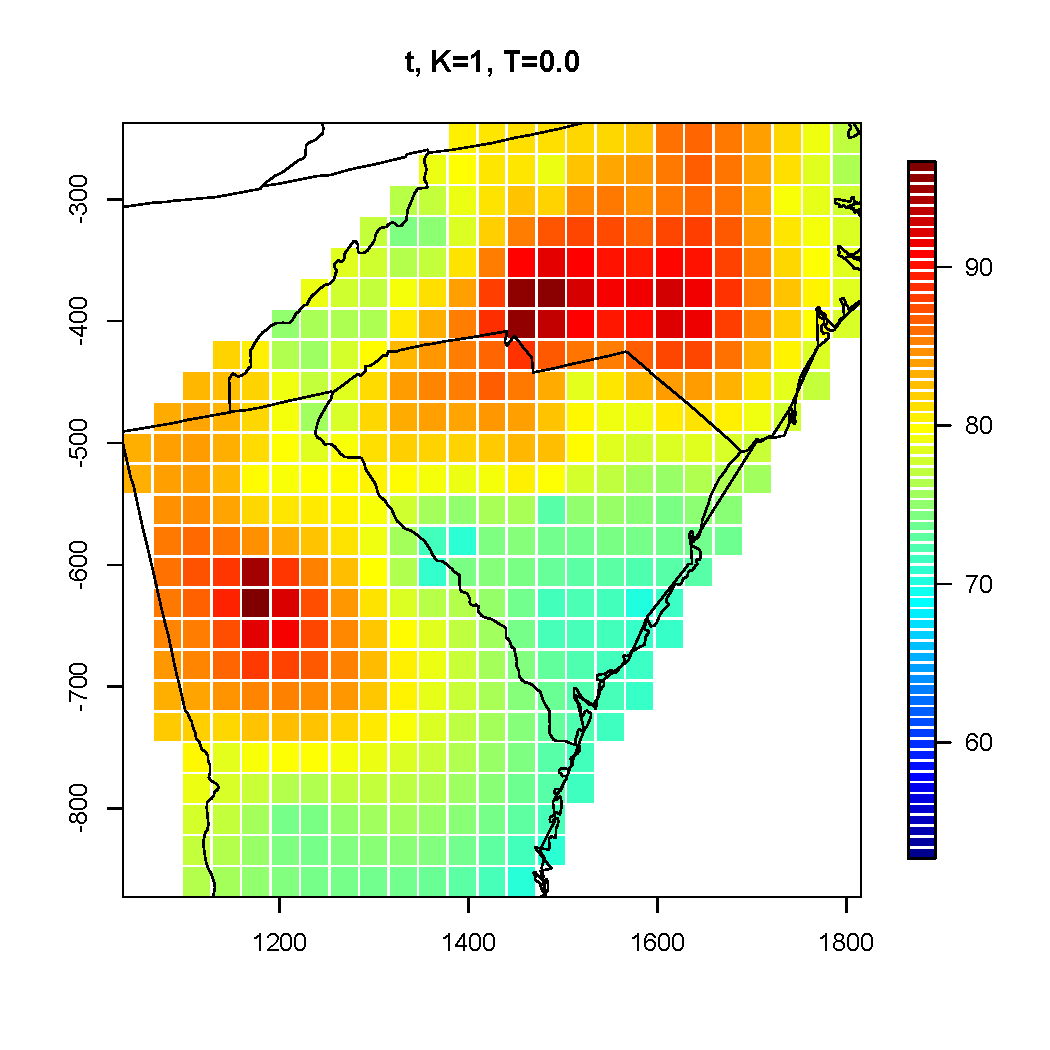
\includegraphics[width=.5\linewidth]{./plots/quantile-99-t10.pdf}
%     \caption{Predicted 99th quantile using Gaussian and $t$}
% \end{figure}
% \end{frame}

% \begin{frame}{Predicted 99th quantile}
% \centering
% \begin{figure}
%     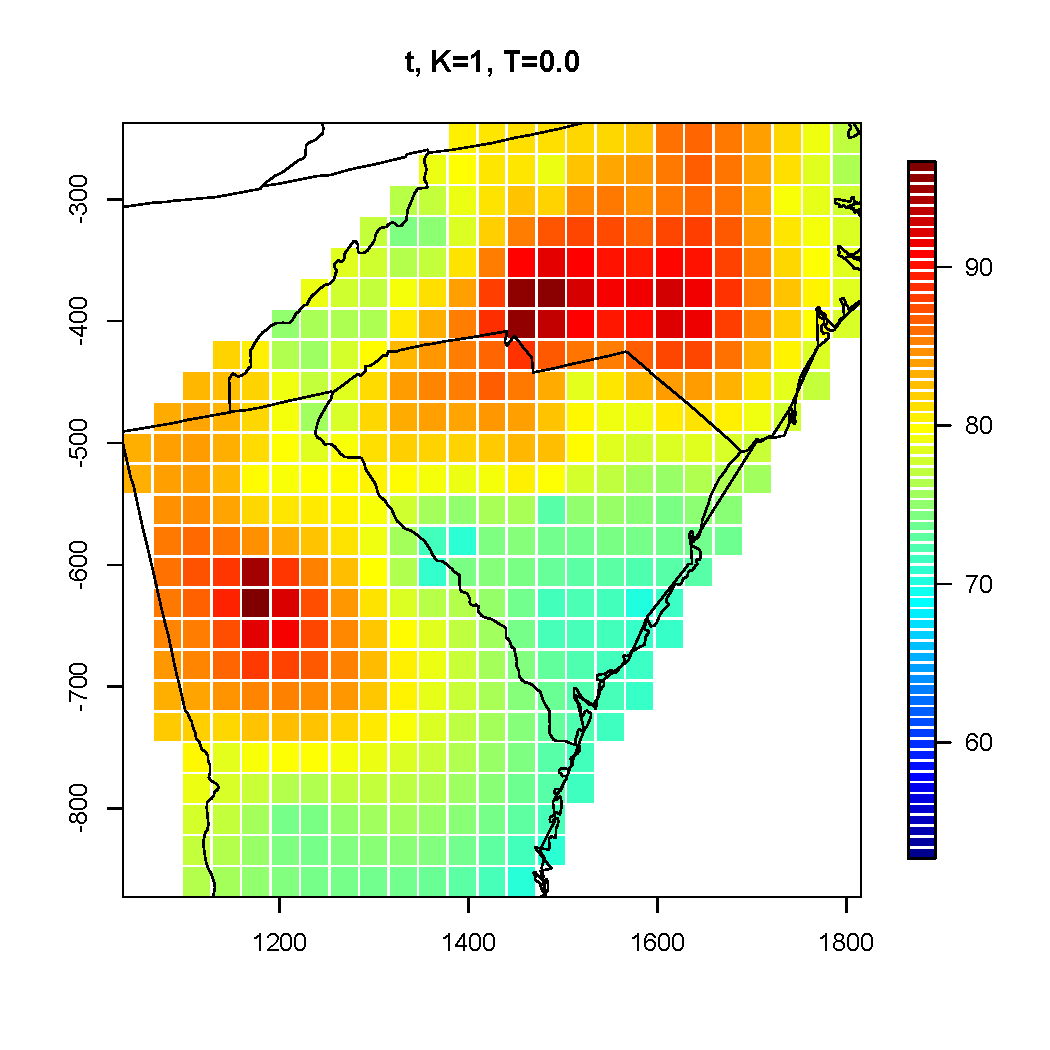
\includegraphics[width=.5\linewidth]{./plots/quantile-99-t10.pdf}
%     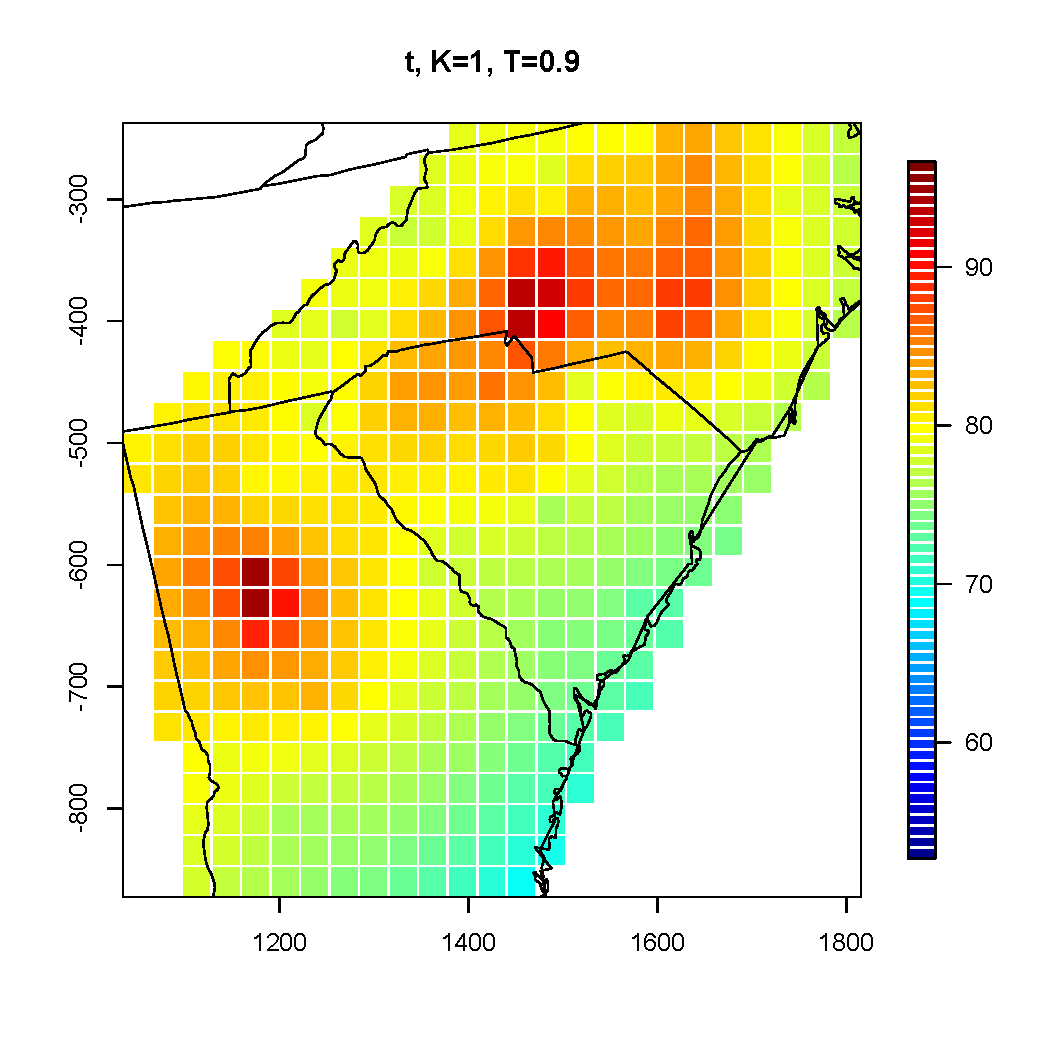
\includegraphics[width=.5\linewidth]{./plots/quantile-99-t19.pdf}
%     \caption{Predicted 99th quantile using $t$ and $t$ thresholded at $T=0.9$}
% \end{figure}
% \end{frame}

% \begin{frame}{Probability of exceedance}
% \centering
% \begin{figure}
%     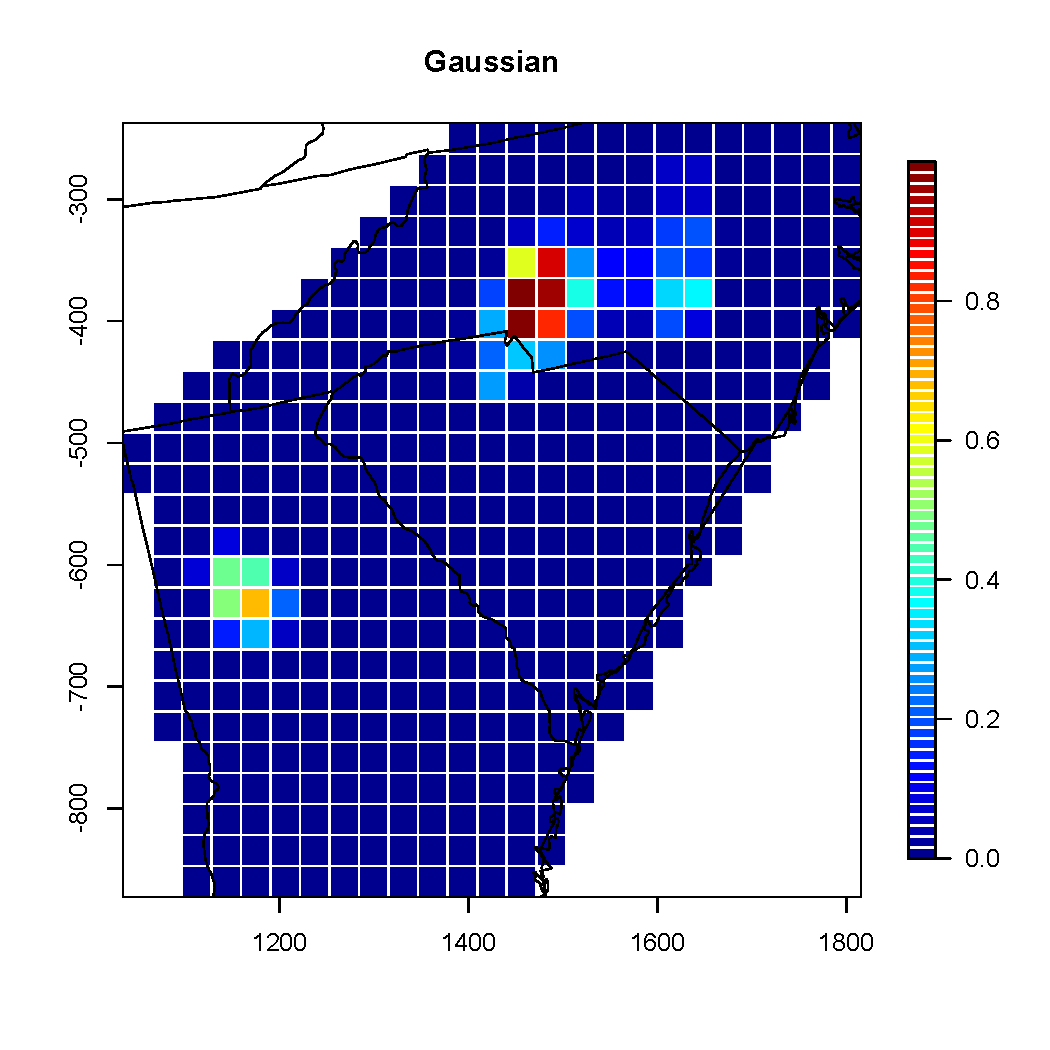
\includegraphics[width=.5\linewidth]{./plots/p-exceed-std-gau.pdf}
%     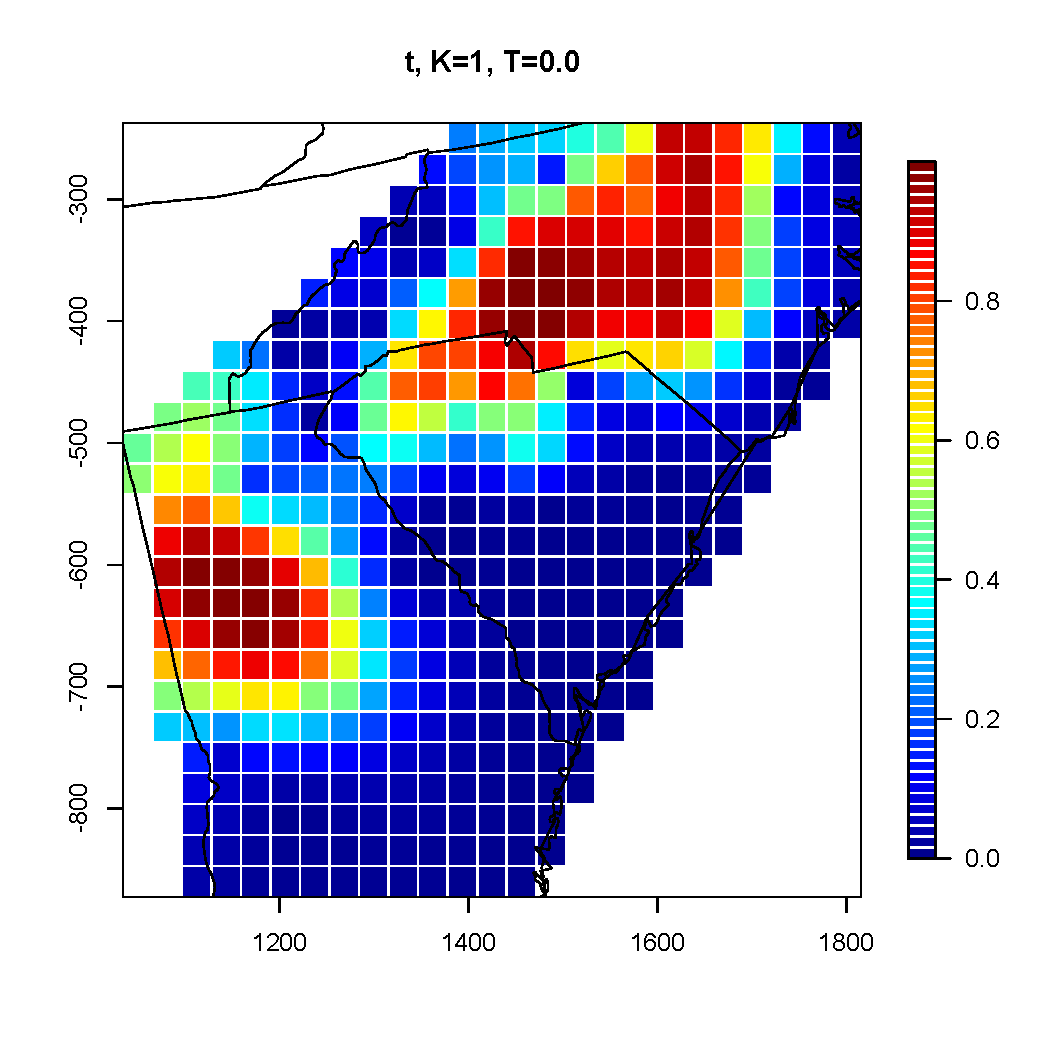
\includegraphics[width=.5\linewidth]{./plots/p-exceed-std-t10.pdf}
%     \caption{Probability of exceeding the 75 ppb ozone standard using Gaussian and $t$}
% \end{figure}
% \end{frame}

% \begin{frame}{Probability of exceedance}
% \centering
% \begin{figure}
%     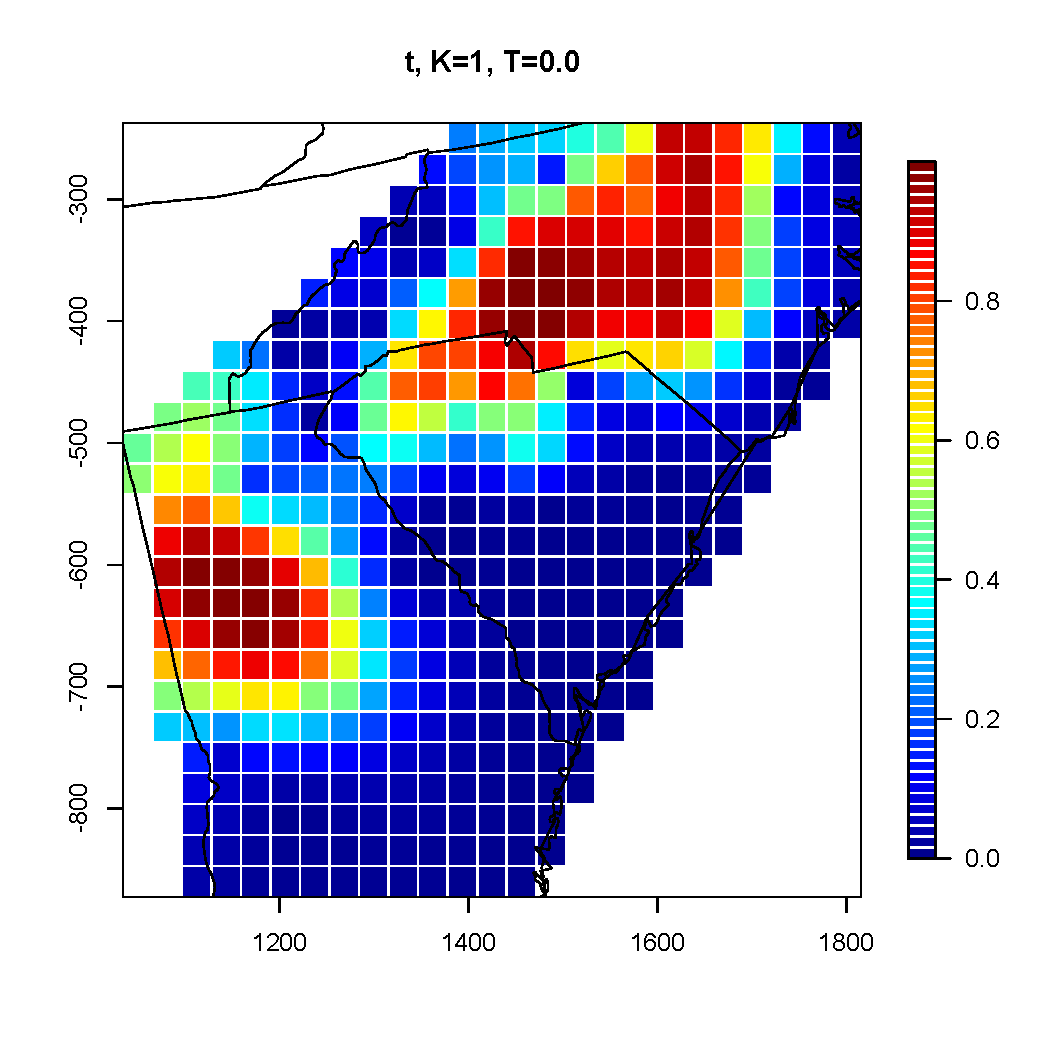
\includegraphics[width=.5\linewidth]{./plots/p-exceed-std-t10.pdf}
%     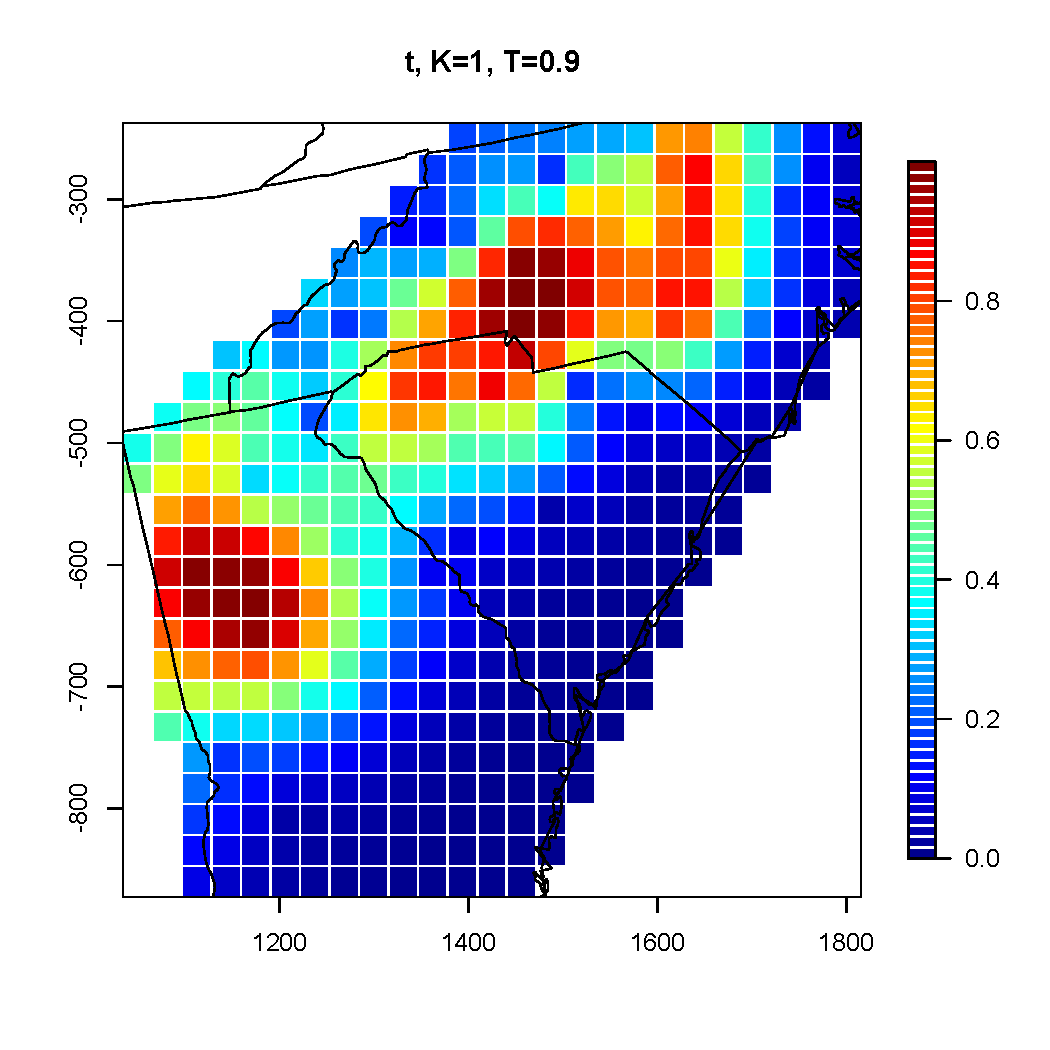
\includegraphics[width=.5\linewidth]{./plots/p-exceed-std-t19.pdf}
%     \caption{Probability of exceeding the 75 ppb ozone standard using $t$ and $t$ thresholded at $T=0.9$}
% \end{figure}
% \end{frame}

\begin{frame}{Discussion and future work}
  \begin{itemize} \setlength{\itemsep}{0.5em}
    \item Improvement of model performance when using partitioned models
    \item Thresholding makes results worse
    \begin{itemize}
      \item Possible numerical instability due to truncated normal distribution
    \end{itemize}
    \item Different ways to incorporate the temporal dependence
    \begin{itemize}
    	\item Three dimensional covariance model for $v_t(\bs)$ (e.g. Huser and Davison, 2014)
    \end{itemize}
    \item Different partition structure
    \begin{itemize}
      \item Distance weighting for each knot vs indicator functions
    \end{itemize}
    \item Knot selection
    \begin{itemize}
      \item Possible prior on the probability a knot is in the spatial domain
    \end{itemize}
  \end{itemize}
\end{frame}

\begin{frame}{Spatial binary regression}
  \begin{itemize} \setlength{\itemsep}{0.5em}
    \item We observe $Y_i = I[Z(\bs_i) > T]$, an indicator variable that a continuous latent variable has exceeded a pre-specified threshold $T$.
    \item We model $\Pr[Y_i = 1]$
    \item Common examples:
    \begin{itemize}
      \item Logistic regression
      \begin{align*}
        \Pr[Y_i = 1] = \frac{ \exp(\bX(\bs_i) \bbeta) }{ 1 + \exp(\bX(\bs_i) \bbeta)}
      \end{align*}
      \item Probit regression
      \begin{align*}
        \Pr[Y_i = 1] = \Phi[\bX(\bs_i) \bbeta]
      \end{align*}
      where $\Phi$ is the standard normal distribution function
    \end{itemize}
  \end{itemize}
\end{frame}

\begin{frame}{Spatial binary regression}
  \begin{itemize} \setlength{\itemsep}{0.5em}
    \item Logistic and probit regression amount to modeling
    \begin{align*}
      \Pr[Y_i = 1] = g[\bX(\bs_i) \bbeta]
    \end{align*}
    where $g[\cdot]$ is a link function transforming from $\calR$ to $(0, 1)$.
    \item Wang and Dey (2010): Generalized extreme value link function
    \begin{align*}
      g[\bx(\bs_i) \bbeta] = 1 - \exp\left[-(1 + \xi \bX_i \bbeta)^{-1 / \xi} \right]
    \end{align*}
  \end{itemize}
\end{frame}

\begin{frame}{Spatial binary regression}
  \begin{itemize} \setlength{\itemsep}{0.5em}
    \item Proposed method will
    \begin{itemize}
      \item use the GEV link function
      \item use the hierarchical likelihood from Reich and Shaby (2012)
    \end{itemize}
    \item Model parameters fit using MCMC
  \end{itemize}
\end{frame}

\begin{frame}{Spatial binary regression}
  \begin{itemize} \setlength{\itemsep}{0.5em}
    \item We fit parameters $\xi$ and $\beta$ in order to transform the data to GEV(1, 1, 1) marginal distributions.
    \item Using the link function
    \begin{align*}
      p_i = 1 - \exp \left[-(1 + \xi \bX(\bs_i) \bbeta)^{-1/\xi}\right]
    \end{align*}
    we set the latent variable $z_i = -\frac{1}{\log(1 - p_i)}$
    \item Then we evaluate the joint likelihood using $z_i$.
  \end{itemize}
\end{frame}

\begin{frame}{Likelihood function}
  \begin{itemize} \setlength{\itemsep}{0.5em}
    \item We use a multivariate generalized extreme value distribution with asymetric Laplace deendence function given by
    \footnotesize{
    \begin{align*}
      G(\bz) = \Pr[Z_1 < z_z, \ldots, Z_n < z_n] = \exp\left\{ - \sum_{l = 1}^{L} \left[ \sum_{i = 1}^n \left( \frac{ w_l(\bs_i) }{ z_i } \right)^{ 1 / \alpha} \right]^\alpha \right\}
    \end{align*}
    }
    where
    \begin{itemize}
      \item $w_l$ is a weighting function subject to the constraint that $\sum_{l = 1}^L w_l = 1$.
      \item $\alpha$ controls spatial dependence
      \begin{itemize}
        \item $\alpha = 0$ is strong dependence
        \item $\alpha = 1$ is joint independence
      \end{itemize}
    \end{itemize}
  \end{itemize}
\end{frame}

\begin{frame}{Weighting function}
  \begin{itemize} \setlength{\itemsep}{0.5em}
    \item We use the Gaussian weights proposed by Reich and Shaby (2012) given by
    \footnotesize{
    \begin{align*}
      w_l(\bs_i) = \frac{ \exp\left[ -0.5 \left( \frac{ || \bs - \bv_l || }{ \rho} \right)^2 \right]}{ \sum_{l = 1}^L \exp\left[ -0.5 \left( \frac{ || \bs - \bv_l || }{ \rho} \right)^2 \right] }
    \end{align*}
    }
    where
    \begin{itemize}
      \item $\bv_l$ are spatial knots
      \item $\rho$ is a bandwidth term for the kernel function
    \end{itemize}
  \end{itemize}
\end{frame}

\begin{frame}{Joint likelihood}
  \begin{itemize} \setlength{\itemsep}{0.5em}
    \item Let $K_t = \sum_{i = 1}^n Y_{it}$ be the number of exceedances that occur on day $t$.
    \item Rearrange the sites so
    \begin{itemize}
      \item $Y_1, \ldots, Y_K$ are the observations where $Y(\bs_i) = 1$
      \item $Y_{K+1}, \ldots, Y_n$ are the observations where $Y(\bs_i) = 0$
    \end{itemize}
    \item Then for $K = 0, 1, 2$
    {\scriptsize
    \begin{align*}
      \Pr(Y_1 = y_1, \ldots, Y_n = y_n) = \left\{ \begin{array}{ll}
        G(\bz)  & K = 0\\
        G(\bz_{(1)}) - G(\bz) & K = 1\\
        G(\bz_{(12)}) - G(\bz_{(1)}) - G(\bz_{(2)}) + G(\bz) & K =2
      \end{array}\right.
    \end{align*}
    }
    where $G(\bz_{(1)} = \Pr(Z_2 < z_2, \ldots, Z_n < z_n)$.
    \item $K > 2$ can be derived similarly
  \end{itemize}
\end{frame}

% TODO: more about this model for sure
\begin{frame}{Non-stationary covariance for extreme values}
  \begin{itemize} \setlength{\itemsep}{0.5em}
    \item Knot-specific bandwidth
  \end{itemize}
\end{frame}

\begin{frame}{Joint likelihood}
  \begin{itemize} \setlength{\itemsep}{0.5em}
    \item For small $K$, we can evaluate the likelihood directly.
    \item For large $K$, we use the hierarchical model of Reich and Shaby (2012).
  \end{itemize}
\end{frame}

\begin{frame}{Thesis outline}
  \begin{itemize} \setlength{\itemsep}{0.5em}
    \item Chapter 1: Extreme value theory \alert{August 2015}
    \item Chapter 2: Spatiotemporal model for extreme value analysis based on the skew-$t$ distribution \alert{February 2015}
    \item Chapter 3: Spatial binary regression \alert{May / June 2015}
    \item Chapter 4: Non-stationary covariance through knot-specific bandwidth \alert{August 2015}
  \end{itemize}
\end{frame}

\begin{frame}{Questions}
  \begin{itemize} \setlength{\itemsep}{0.5em}
    \item Questions?
    \item Thank you for your attention.
    \item Acknowledgment: This work was funded by EPA STAR award R835228
  \end{itemize}
\end{frame}

\begin{frame}{References}
  \begin{itemize} \setlength{\itemsep}{0.5em}
    \item Demarta, S. and McNeil, A. J. (2007) The $t$ copula and related copulas. {\it International Statistical Review}, {\bf 73}, 111--129.
    \item Huser, R. and Davison, A. C. (2014) Space-time modelling of extreme events. {\it Journal of the Royal Statistical Society: Series B (Statistical Methodology)}, {\bf 76}, 439--461.
    \item Padoan, S. A. (2011) Multivariate extreme models based on underlying skew-$t$ and skew-normal distributions. {\it Journal of Multivariate Analysis}, {\bf 102}, 977--991.
    \item Zhang, H. and El-Shaarawi, A. (2010) On spatial skew-Gaussian processes and applications. {\it Environmetrics}, {\bf 21}, 33--47.
  \end{itemize}
\end{frame}

\end{document}